\chapter{Accelerarea hardware}
\label{chapter:acc}

%=============================================================================
% KERNEL ASPECTE SPECIFICE
%=============================================================================
\section{Aspecte specifice în implementarea kernelurilor}
\label{sec:kernel-aspects}

Procesorul ConnexArray permite lucrul atât cu tipuri de date fracționare în
virgulă fixă, cât și în virgulă mobilă, cu diferențe în ceea ce privește
precizia rezultatelor și timpul de calcul. 

Datele în virgulă fixă au avantajul că se procesează rapid, operațiile de
adunare, scădere, înmulțire sau depalasare efectuate pe ele durând doar un ciclu
de ceas, la fel ca în cazul numerelor întregi. În realitate, procesorul nu
diferențiază numerele întregi de numerele fracționare în virgulă fixă, lăsând în
sarcina programatorului interpretarea acestora în funcție de context. Pentru
conversia din date în virgulă mobilă, cum sunt cele utilizate în general în
limbajul C++, la cele în virgulă fixă necesare acceleratorului ConnexArray, este
necesară o pre-scalare cu un anumit factor, ales în funcție de gama dinamică a
numerelor, și o conversie la tipul de date întreg fără semn pe 16 biți
(\code{uint16\_t}). \\

În ceea ce privește datele în virgulă mobilă, nu există suport hardware pentru
acestea, iar calculul se bazează pe o emulare software, motiv pentru care
operațiile în virgulă mobilă pe procesor sunt foarte lente (de exemplu, o
înmulțire între două date în virgulă mobilă poate consuma până la 50 de cicli de
ceas). \\

Prin urmare, având în vedere că performanța programului este punctul principal
de interes și că datele de intrare au o gamă dinamică destul de mică, în
intervalul $(-2, 2)$, am ales reprezentarea datelor în virgulă fixă. \\

Funcționarea cozilor pentru comunicarea cu acceleratorul a fost explicată în
Secțiunea~\ref{sec:cnx-arr}, dar este important de precizat un aspect
referitor la tipurile de date cu care lucrează. Un rezultat urmat în urma unei
procesări pe accelerator poate fi citit fie din memoria sa locală, prin metoda
\code{writeDataToArray}, caz în care citirea se face prin intermediul cozii
\code{readFIFO}, fie, dacă acest rezultat este urmarea unei reducții,
poate fi citit direct din coada \code{reductionFIFO} cu ajutorul metodei
\code{readReduction}. În primul caz, rezultatele vor fi pe 16 biți, fără semn,
urmând ca interpretarea lor cu semn să se facă în funcție de factorul cu care au
fost scalate datele, iar în al doilea caz rezultatul va fi pe 32 biți, cu semn. \\

În esență, există două considerente principale care trebuie luate în calcul în
conceperea unui kernel:
\begin{itemize}
  \item \textbf{Gestionarea datelor}, care presupune aranjarea datelor în
  memoria locală a acceleratorului, eventuala lor împărțire în blocuri de date
  care vor fi procesate în aceeași execuție a kernelului, când se face
  conversia lor din virgulă mobilă în virgulă fixă (și invers) și unde, momentul
  scrierii și citirii lor.

  \item \textbf{Algoritmul propriu-zis} implementat de kernel, care asumă deja
  o anumită aranjare anterioară a datelor.
\end{itemize}

Deși primul considerent este legat mai mult de programul principal și nu de
mediul de lucru OPINCAA, el este puternic corelat cu procesarea pe accelerator,
deci nu poate fi tratat separat și poate avea un impact major asupra
performanței toate a procesării.  \\

Un alt factor care trebuie luat în considerare este cel al dimensiunii
tablourilor cu care se operează. În cazul ideal, performanțele maxime se obțin
dacă acestea au ca dimensiuni puteri ale lui 2, care va facilita aranjarea lor
pe liniile de procesare. Memoria locală, la modul general, are o capacitate de M
linii a câte N elemente, unde N este numărul de elemente de procesare, structură
ilustrată în Figura~\ref{fig:local-storage-struct}. Se observă cum un anumit
PE\textsubscript{i} are acces la elementele LS[k][i] din memoria locală, unde $i
= \overline{0, N-1}$, $k = \overline{0, M-1}$. În cazul de față, acceleratorul
are o configurație cu N = 128 elemente de procesare și o memorie locală cu M = 1024
linii. \\

\begin{figure}[h]
    \centering
    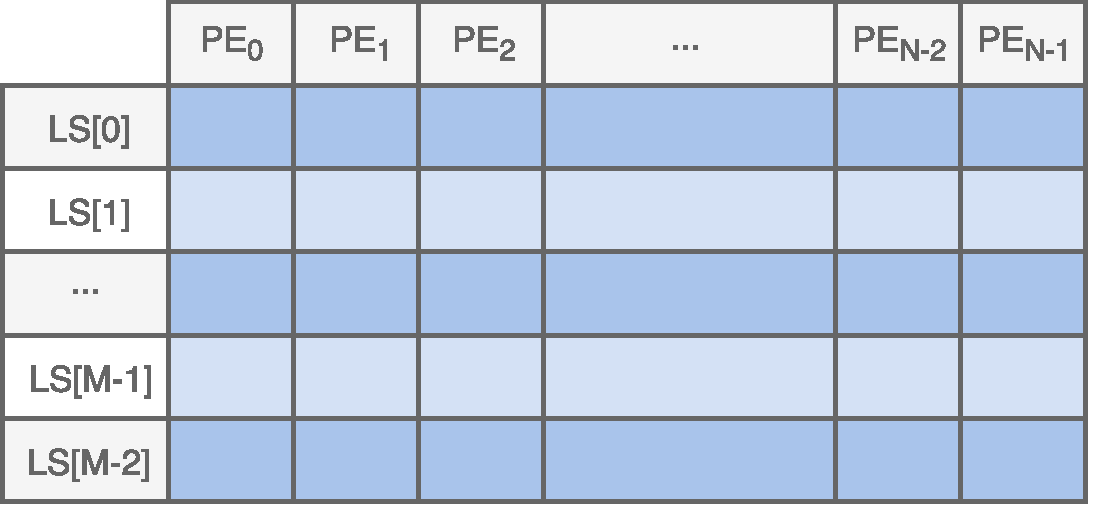
\includegraphics[width=0.6\textwidth]{src/img/local-storage-struct}
    \caption{Structura memoriei locale a acceleratorului ConnexArray}
    \label{fig:local-storage-struct}
\end{figure}

Observăm că cele mai importante limitări în procesarea datelor pe accelerator
constă în pregătirea datelor de intrare și de ieșire și capacitatea memoriei
locale, care constrânge numărul de date care pot fi procesate într-o execuție a
unui kernel. Prin urmare, dacă avem un număr de date de intrare de procesat mai
mare decât capacitatea memoriei locale a acceleratorului, acestea trebuie
împărțite în blocuri de procesare de dimensiune mai mică (și, preferabil, de
dimensiune egală).  Avantajul procesării
în blocuri cât mai mari de date este faptul că operațiile de I/O vor fi mai
puține și se va elimina, astfel, un \textit{overhead} important. \\

În plus, un avantaj este dat de faptul că putem pregăti datele de intrare pentru
procesarea blocului următor (sau realiza alte operații) în timpul în care, în
mod normal, am aștepta datele de ieșire de la accelerator. Acest lucru se poate
face fie în același fir de execuție, întrucât lansarea în execuție a unui kernel
nu este o operație blocantă, spre deosebire de citirea datelor, sau lansarea
unui alt fir de execuție care să realizeze procesarea dorită și, dacă este
necesar, sincronizarea lui cu firul principal de execuție. \\

În continuare, vom prezenta câteva soluții de realizare a kernelurilor pentru
problemele identificate în modulul \code{gr-doa} care au la bază înmulțiri de
tablouri de date. Astfel, Secțiunea~\ref{sec:kernel-mult} prezintă înmulțirea
vectorilor de numere complexe, Secțiunea~\ref{sec:kernel-mult-array} dezvoltă
înmulțirea unui vector cu o matrice pătratică, în
Secțiunea~\ref{sec:kernel-mult-chain} a fost elaborat un algoritm pentru o
înmulțire înlănțuită dintre un vector, o matrice pătratică și un vector, iar în
Secțiunea~\ref{sec:kernel-autocorr} este prezentată o modalitate de realizare a
autocorelației unui semnal de intrare. În final, am descris modalitatea de
integrare a acestor kerneluri în mediul de dezvoltare GNU Radio în
Secțiunea~\ref{sec:kernel-integrate}.

%=============================================================================
% KERNEL VECTOR x VECTOR NR. COMPLEXE
%=============================================================================
\section{Înmulțirea vectorilor de numere complexe pe procesorul ConnexArray}
\label{sec:kernel-mult}

Considerăm, mai întâi, un caz general în care înnmulțim un vector linie X cu un
vector coloană Y, de aceeași dimensiune N pe care, pentru simplitate, o presupunem
egală jumătate din numărul de elemente de procesare ale acceleratorului.
\begin{equation}
    \bm{X}
    \overset{\Delta}{=}
    \begin{bmatrix}
       x_0   &   x_1   &   \hdots   &   x_{N-1}
    \end{bmatrix}
\end{equation}
\begin{equation}
    \bm{Y}
    \overset{\Delta}{=}
    \begin{bmatrix}
       y_0   &   y_1   &   \hdots   &   y_{N-1}
    \end{bmatrix}^T
\end{equation}

Vectorii conțin numere complexe, deci elementele lor vor fi de forma:
\begin{equation}
x_i = a_i + jb_i, \quad i = \overline{0, N-1}
\end{equation}
\begin{equation}
y_{i} = a'_{i} + jb'_{i}, \quad i = \overline{0, N-1}
\end{equation}

Rezultatul înmulțirii celor doi vectori va fi o matrice cu un singur element
complex.
\begin{equation}
    \bm{R}
    \overset{\Delta}{=}
    \bm{X}\bm{Y}
    =
    \begin{bmatrix}
       \displaystyle{\sum_{i=0}^{N-1} x_iy_i}
    \end{bmatrix}
    = 
    \begin{bmatrix}
       \displaystyle{\sum_{i=0}^{N-1} (a_ia'_i - b_ib'_i) + j\sum_{i=0}^{N-1}
       (a_ib'_i - a_ib'_i)}
    \end{bmatrix}
\end{equation}

Propunem, pentru calculul rezultatului, metoda de aranjare a elementelor din
Figura \ref{fig:complex-mult}, care figurează și următorii pași de procesare:

\begin{enumerate}
\item Elementele din primul vector sunt încărcate în
locații succesive din memoria locală a acceleratorului, părțile lor reale
alternând cu cele imaginare, iar apoi sunt transferate într-un registru (în
cazul de față R1), procedând în mod asemănător și pentru cel de-al doilea
(pentru acesta, vor fi transferate în registrul R2). În acest mod, părțile reale ale elementelor celor
doi vectori se vor afla în PE cu număr de ordine par, iar cele imaginare în PE
cu număr de ordine impar.

\item Efectuăm înmulțirea dintre conținutul registrelor R1 și R2, obținând
astfel produsele necesare pentru calculul părții reale a rezultatului, care
vor fi păstrate în registrul R3. 

\item Se inversează semnul produselor de părți imaginare din registrul R3 doar
pe PE-urile impare.

\item Se aplică o reducție pe registrul R3, obținând partea reală a
rezultatului final.

\item Pentru a calcula partea imaginară a rezultatului, va trebui să aducem
părțile imaginare ale elementelor din cel de-al doilea vector în aceleași PE-uri
cu părțile reale ale primului, păstrând rezultatul deplasării în registrul R4.

\item Reciproc, părțile reale ale elementelor celui de-al doilea vector sunt
aduse în aceleași PE-uri cu părțile imaginare ale elementelor primului vector și
stocăm rezultatul deplasării în registrul R5.

\item Efectuăm o înmulțire între registrele R1 și R4 și suprascriem rezultatul
în registrul R4.

\item Efectuăm o înmulțire între registrele R2 și R5 și suprascriem rezultatul
în registrul R5.

\item În acest moment, avem produsele necesare pentru calculul părții imaginare a
rezultatului final. Observăm, din Figura \ref{fig:complex-mult}, că vom obține
rezultate de interes doar în PE-urile cu index par pentru registrul R4 și în
cele cu index impar pentru cele din registrul R5, deci, pentru un rezultat
corect, putem muta doar conținutul registrului R5 din PE-urile impare în
registrul R4.

\item Toate produsele parțiale pentru partea imaginară a rezultatului se află
acum în registrul R4 și vom finaliza calculul acesteia prin aplicarea unei
reducții pe acesta.
\end{enumerate}

\begin{figure}[H]
    \centering
    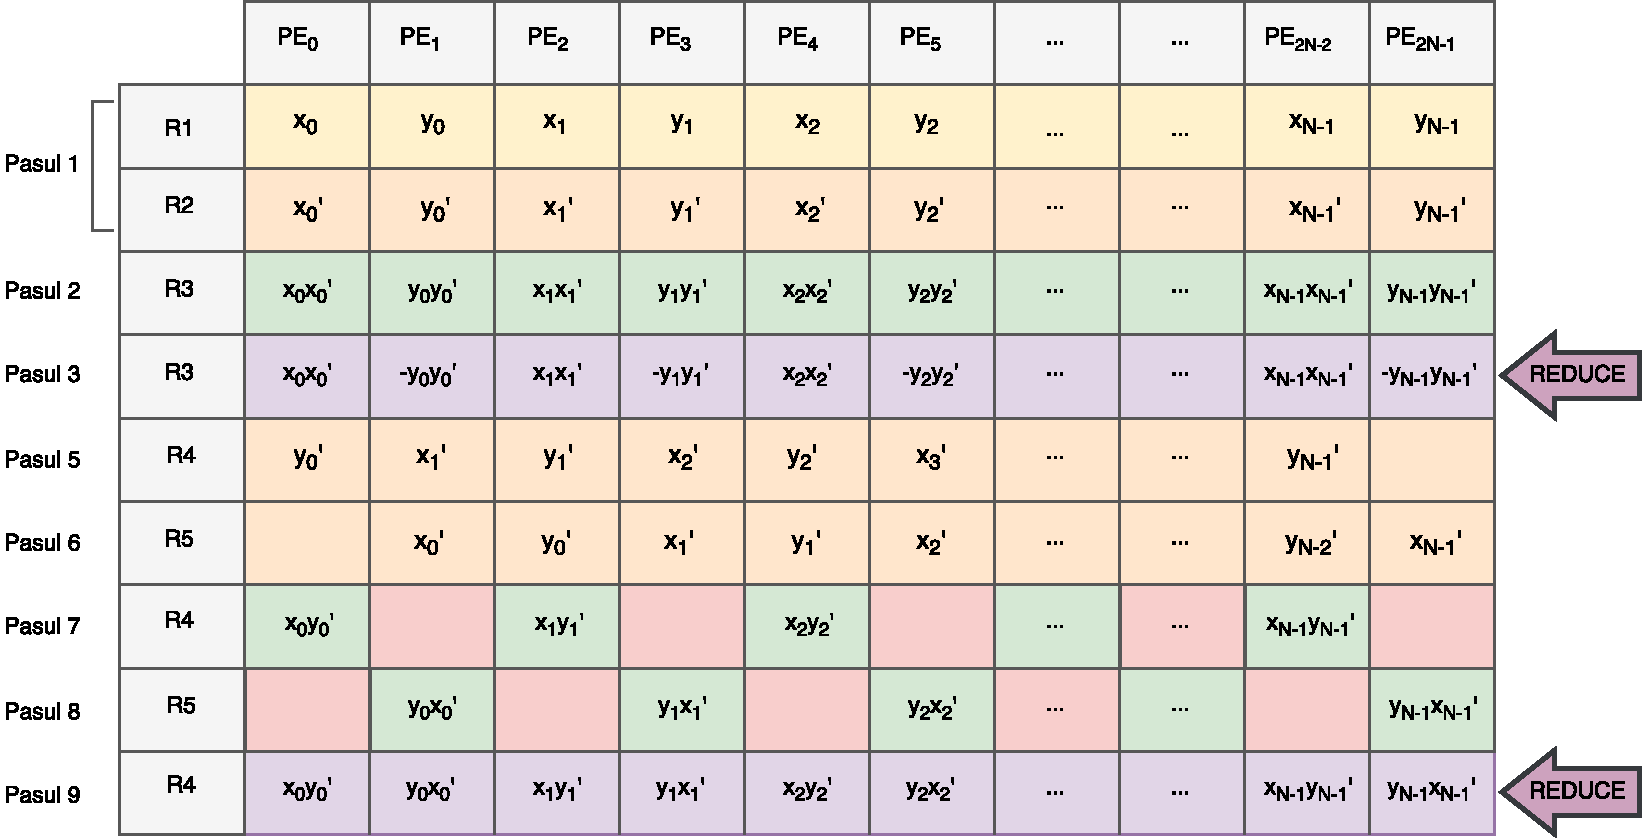
\includegraphics[width=1\textwidth]{src/img/complex-mult-arrow}
    \caption{Înmulțirea a doi vectori de numere complexe pe ConnexArray}
    \label{fig:complex-mult}
\end{figure}

Kernelul care implementează algoritmul descris se află în Anexa \ref{sec:kernel-mult-arr} Pentru
eficiență, pașii nu se execută în ordinea explicată mai sus ci, de exemplu, se
pot combina pașii 3 și 9 pentru reducerea timpului de calcul. O îmbunătățire
adițională poate consta în rearanjarea instrucțiunilor astfel încât să se evite
efectuarea unui \code{NOP} acolo unde este posibil, dar acest lucru reduce
lizibilitatea codului, motiv pentru care va fi realizată doar în implementare. \\

În cazurile destul de comune întâlnite în practică în care dimensiunea unui
vector (N) va fi mai mică decât numărul de PEs disponibile, putem, să efectuăm
mai multe înmulțiri în aceeași execuție a kernelului. Modificarea va consta în
faptul că reducția va trebui, în acest caz, efectuată în blocuri de dimensiune
$2 \cdot N$. \\

În cazul contrar, în care N depășește capacitatea unei linii a aceleratorului,
algoritmul propus poate funcționa în continuare dacă la ,,pregătirea'' datelor
de ieșire luăm în considerare faptul că mai multe rezultate de reducție trebuie
însumate pentru formarea unui element al matricei de ieșire. Dacă N nu este un
multiplu al capacității liniilor de procesare, elementele rămase neocupate
dintr-o linie să fie inițializate cu zero pentru a nu afecta rezultatul
reducției, procedeu cunoscut sub numele de \textit{zero padding}.

%=============================================================================
% KERNEL VECTOR x MATRICE
%=============================================================================
\section{Kernel pentru înmulțirea unui vector cu o matrice}
\label{sec:kernel-mult-array}

Unul dintre punctele critice ale implementării algoritmului MUSIC a fost găsit
în blocul \textbf{MUSIC Linear Array}, detaliat în
Secțiunea~\ref{ssec:music-lin-array}, la calculul spectrului MUSIC utilizând
formula de mai jos.
\begin{equation}
    P_{MUSIC}(\theta) =
        \frac{1}
             {\bm{a}^H(\theta)\bm{V}_N\bm{V}_N^H\bm{a}(\theta)} \\
\label{eq:music-spectrum-kernel}
\end{equation}

Avem de a face, prin urmare, cu o înmulțire înlănțuită dintre un vector linie
$\bm{a}^H(\theta)$ de lungime M, o matrice pătratică formată din produsul
$\bm{V}_N\bm{V}_N^H$ pe care o vom nota $V_{N_{sq}}$, de dimensiune $M \times M$
și un vector coloană $\bm{a}(\theta)$ de lungime M. Vom nota rezultatul primei
părți a înmulțirii $X_M \overset{\Delta}{=} \bm{a}^H(\theta)\bm{V}_{N_{sq}}$. \\

Am decis să calculăm $X_M$ pe procesorul SIMD și partea finală
$X_M\bm{a}(\theta)$ va fi lăsată ca discuție din considerente de
performanță, urmând  a stabili dacă este mai eficient să fie calculată pe
procesorul ARM sau dacă este de preferat varianta efectuării întregului produs
de trei matrice pe procesorul ConnexArray, care va fi descrisă în Secțiunea
\ref{sec:kernel-mult-chain}. \\

Mai întâi, considerăm cazul general al înmulțirii dintre un vector
linie de lungime M cu o matrice pătratică de dimensiune $M \times M$, din care
rezultă un vector linie de lungime M.
\begin{equation}
    X_M
    \overset{\Delta}{=}
    \begin{bmatrix}
        \overline{a}_0   &   \overline{a}_1   &   \hdots   &   \overline{a}_{M-1}
    \end{bmatrix}
    \begin{bmatrix}
        v_{0,0}   &   v_{0,1}   &   \hdots   &   v_{0,M-1} \\
        v_{1,0}   &   v_{1,1}   &   \hdots   &   v_{1,M-1} \\
        \vdots    &   \vdots    &   \ddots   &   \vdots    \\
        v_{M-1,0} &   v_{M-1,1} &   \hdots   &   v_{M-1,M-1}
    \end{bmatrix}
\end{equation}
\begin{equation}
    X_M
    =
    \begin{bmatrix}
        \displaystyle{\sum_{i=0}^{M-1} \overline{a}_iv_{i,0}} & 
        \displaystyle{\sum_{i=0}^{M-1} \overline{a}_iv_{i,1}} & 
        \hdots &
        \displaystyle{\sum_{i=0}^{M-1} \overline{a}_iv_{i,M-1}}
    \end{bmatrix}
    , unde
\end{equation}
\begin{equation}
a_i = x_i + jy_i, \quad i = \overline{0, M-1}
\end{equation}
\begin{equation}
\overline{a}_i = x_i - jy_i \overset{not}{=} x_i + j\overline{y}_i, \quad i = \overline{0, M-1}
\end{equation}
\begin{equation}
v_{i,k} = x_{i,k} + jy_{i,k}, \quad i = \overline{0, M-1}, k = \overline{0, M-1}
\end{equation}

Rezultatul poate fi scris în continuare:
\begin{equation}
X_M
=
\begin{bmatrix}
  \displaystyle{\sum_{i=0}^{M-1} (x_ix_{i,0} - \overline{y}_iy_{i,0}) + 
               j\sum_{i=0}^{M-1} (x_iy_{i,0} + \overline{y}_ix_{i,0})} \\ 
  \displaystyle{\sum_{i=0}^{M-1} (x_ix_{i,1} - \overline{y}_iy_{i,1}) + 
               j\sum_{i=0}^{M-1} (x_iy_{i,1} + \overline{y}_ix_{i,1})} \\
  \hdots \\
  \displaystyle{\sum_{i=0}^{M-1} (x_ix_{i,M-1} - \overline{y}_iy_{i,M-1}) + 
               j\sum_{i=0}^{M-1} (x_iy_{i,M-1} + \overline{y}_ix_{i,M-1})} \\ 
\end{bmatrix}^T
\label{eq:expresie-inmultire}
\end{equation}

În mod evident, implementarea acestui produs se poate face extinzând algoritmul
de înmulțire a doi vectori, unul linie și celălalt coloană, de aceeași
dimensiune, deoarece înmulțirea unui vector cu o matrice constă, de fapt, în
înmulțirea vectorului de intrare cu alți vectori formați din coloanele matricei
de intrare, după cum se poate observa în Figura \ref{fig:cnx-vec-mat}. \\

\begin{figure}[h]
    \centering
    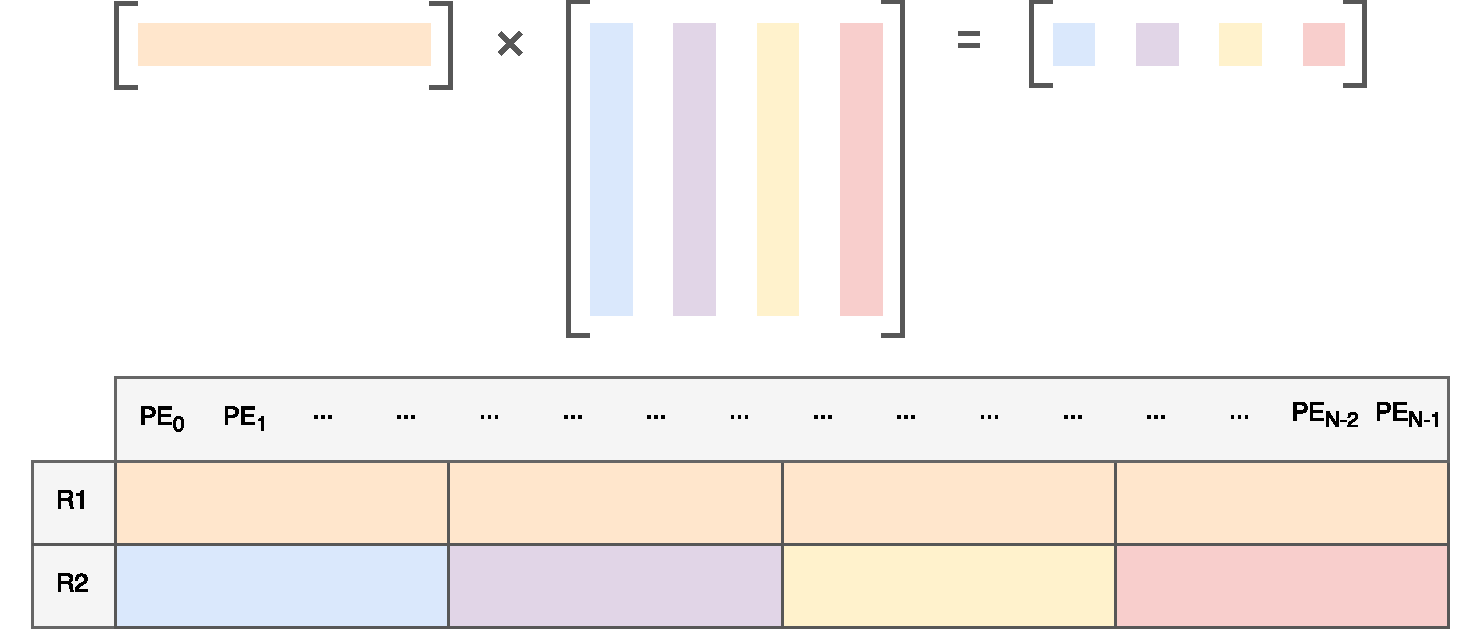
\includegraphics[width=0.7\textwidth]{src/img/vec-matrix}
    \caption{Exemplu de aranjare a elementelor în ConnexArray pentru o înmulțire
    dintre un vector și o matrice}
    \label{fig:cnx-vec-mat}
\end{figure}

Putem să distingem mai multe variații ale metodei propuse în funcție de numărul
de elemente al matricei. Dacă notăm \code{arr\_size\_c} $= M \times 2$ și
\code{mat\_size\_c} $= M \times M \times 2$ numărul de elemente în care am
separat părțile reale și imaginare ale matricei, respectiv vectorului de intrare
și \code{vector\_array\_size} numărul de elemente de procesare ale
acceleratorului, avem următoarele posibilități de aranjare a datelor de intrare
în memoria locală a acceleratorului:

\begin{enumerate}[label=\alph*., ref=\alph*]
  \item \label{enum:kernel-a} \code{mat\_size\_c} $\le$
  \code{vector\_array\_size} - în acest caz, cel puțin o matrice poate fi
  încărcată într-o linie din LS, coloană cu coloană.  Deoarece vectorul de
  intrare se înmulțește cu fiecare coloană, el va fi copiat de M ori și stocat
  într-o altă linie din LS. Numărul de înmulțiri dintre vectori linie și matrice
  care pot fi efectuate simultan pe accelerator este egal cu numărul de matrice
  care încap într-o linie de procesare. În Figura \ref{fig:cnx-more-mult} am
  prezentat aranjarea elementelor în ConnexArray în cazul în care se efectuează
  simultan două înmulțiri dintre doi vectori de intrare și aceeași matrice, unde
  $V.col(i)$ reprezintă un vector format din coloana $i$ a matricei de intrare.  
  
  În general, vom dori să efectuăm înmulțiri pe blocuri mai mari de date într-o
  execuție a unui kernel, în care vom ocupa mai multe linii din LS, care vor fi
  apoi aduse, pe rând, în registre și prelucrate în mai multe iterații. Un
  exemplu de aranjare a vectorilor în această situație este prezentat în Figura
  \ref{fig:chunking-a}, în care s-a luat în considerare faptul că elementele nu
  vor ocupa toată capacitatea acceleratorului și trebuie adăugate elemente de
  gardă pentru aliniere (\textit{padding}). Este de ajuns ca matricea să fie
  încărcată într-o singură linie de procesare, restul fiind ocupate cu vectorii
  cu care aceasta se înmulțește.
  
  În practică, pentru un accelerator o capacitate de 128 de elemente de procesare,
  se pot prelucra matrice cu dimensiunea maximă $8 \times 8$ care, în contextul
  algoritmului MUSIC, corespund unei configurații cu cel mult opt antene de
  recepție. 
  
  Vor fi efectuați următorii pași în kernel, corespunzători pseudocodului din
  Listarea \ref{lst:pseudocode-mult-a}:
  \begin{enumerate}[label=\arabic*., ref=\arabic*]
    \item Încărcăm linia cu matricea de intrare într-un registru.
    \item La începutul fiecărei iterații pentru fiecare LS din blocul de
    procesare, încărcăm o linie din LS cu vectori de intrare într-un registru.
    În interiorul fiecărei iterații:
    
    \begin{enumerate}[label*=\arabic*., ref=\arabic*]
      \item Efectuăm înmulțirea dintre registrele din fiecare PE descrisă în
      Secțiunea~\ref{sec:kernel-mult}.
      \item Realizăm reducții în blocuri de câte \code{arr\_size\_c}
      elemente pentru fiecare coloană a fiecărei matrice din linia de procesare.
      \item Incrementăm registrul folosit în adresarea liniilor din LS ce conțin
      vectori și trecem la următoarea iterație pentru fiecare LS din blocul de
      procesare.
    \end{enumerate}
  \end{enumerate}
 
  Codul kernelului care implementează algoritmul descris se află în Anexa
  \ref{sec:kernel-mult-arr-mat}.

  \item \label{enum:kernel-b} \code{mat\_size\_c} $>$ \code{vector\_array\_size} și
  \code{arr\_size\_c} $<$ \code{vector\_array\_size} - în această situație,
  matricea de intrare va ocupa mai multe linii din memoria locală și nu va mai
  fi nevoie să stocăm vectorul de intrare de mai multe ori, ci îl vom refolosi
  pentru fiecare înmulțire cu un set de coloane, după cum este
  ilustrat în Figura \ref{fig:chunking-b}. Din motive de aliniere, vom stoca
  doar coloane întregi într-o linie de procesare și, dacă aceasta va fi
  incompletă, vom adăuga un \textit{padding} până la completarea ei. Poate
  apărea situația în care ultima dintre liniile din LS în care este stocată
  matricea este incompletă, cum este cazul liniei LS[i] din figură, care trebuie
  tratată separat, în toate celelalte linii fiind stocate câte $k$ coloane din
  matricea de intrare. Am considerat că matricea este stocată pe $x$ linii din LS,
  iar vectorii ocupă, în total, $y$ linii din LS.

  Având în vedere notațiile menționate, se vor parcurge următorii pași,
  sintetizați și în pseudocodul din Listarea \ref{lst:pseudocode-mult-b}:
  \begin{enumerate}[label=\arabic*., ref=\arabic*]
    \item Avem $y$ iterații pentru fiecare linie din LS care conține vectori, la
    începutul căreia se aduce câte una dintre ele într-un registru. În
    interiorul fiecărei iterații:
    \begin{enumerate}[label*=\arabic*., ref=\arabic*]
      \item Efectuăm $x-1$ iterații pentru fiecare linie (cu excepția ultimei) din
      LS în care se află stocată matricea, la începutul căreia aceasta se
      transferă într-un registru. În interiorul fiecărei iterații:\\
        - Efectuăm înmulțirea dintre registrele din fiecare PE descrisă în
        Secțiunea~\ref{sec:kernel-mult}. \\
        - Vom realiza câte două reducții pentru fiecare dintre cele k coloane
        dintr-o linie de procesare. 
      \item Ultima linie din LS care conține o parte din matrice va fi tratată
      separat, deoarece este posibil să se efectueze un număr mai mic de reducții.
      De exemplu, în Figura \ref{fig:chunking-b} se vor efectua reducții doar pe
      două blocuri după ce, în prealabil, s-au înmulțit registrele ca într-un caz
      obișnuit. Acest pas este necesar pentru a nu procesa elemente în plus,
      pe care ar trebui apoi să le luăm în calcul la citirea rezultatelor.
    \end{enumerate}
    \item Incrementăm registrul folosit în adresarea liniilor din LS ce conțin
    vectori și trecem la iterația pentru următoarea linie care conține un vector
    de intrare.
  \end{enumerate}
  
  Acest caz corespunde unei configurații care are între 9 și 64 antene de
  recepție, dacă am considerat o configurație ConnexArray cu 128 PEs.

  \item \label{enum:kernel-c} \code{mat\_size\_c} $>$ \code{vector\_array\_size} și
  \code{arr\_size\_c} $>$ \code{vector\_array\_size} - diferența față de cazul
  anterior constă în faptul că o singură coloană din matricea de intrare va
  ocupa mai multe linii din memoria locală, la fel ca și vectorul cu care se
  înmulțește matricea, care va trebui stocat, ca și în cazul precedent, o
  singură dată. Aranjamentul propus este redat în Figura
  \ref{fig:chunking-c}, unde numărul de linii ocupat de o coloană din matrice a
  fost notat $n$, la fel ca și cel ocupat de un vector, iar numărul total de
  linii ocupate de matrice a fost notat $x$.

  Kernelul va implementa următorul algoritm, redat și sub forma unui pseudocod
  în Listarea~\ref{lst:pseudocode-mult-c}:
  \begin{enumerate}[label=\arabic*., ref=\arabic*]
    \item \label{enum:it-vec} Efectuăm câte o iterație pentru fiecare vector
    procesat în execuția curentă.
    \begin{enumerate}[label*=\arabic*., ref=\arabic*]
      \item Efectuăm câte o iterație pentru fiecare coloană a matricei de intrare,
      la începutul căreia se resetează pointerul către o linie dintr-un vector la
      linia inițială. În Figura \ref{fig:chunking-c}, pentru vectorul \code{arr0},
      aceasta este LS[x].
      \begin{enumerate}[label*=\arabic*., ref=\arabic*]
        \item Efectuăm câte o iterație pentru fiecare dintre cele $n$ linii din LS
        care conțin o coloană din matricea de intrare. În interiorul fiecărei
        iterații:\\
          - Încărcăm liniile curente care conțin o parte
          dintr-o matrice și dintr-un vector în registre și le înmulțim.\\
          - Vom reduce o întreagă linie odată, deci este important ca
          \textit{padding}-ul să fi fost făcut cu 0, pentru a nu afecta
          calculele.\\
          - Se incrementează pointerii la matrice și vector și se trece la
          următoarea iterație pentru fiecare coloană a matricei.
        \item La sfârșitul tuturor celor $n$ iterații pentru fiecare coloană a
        matricei de intrare, se incrementează pointerul la vector astfel încât să
        corespundă următorului vector de intrare și se trece la următoarea iterație
        de la Pasul~\ref{enum:it-vec}.
      \end{enumerate}
    \end{enumerate}
  \end{enumerate}
  
  Pentru configurația ConnexArray folosită, în această categorie intră
  procesările pentru sisteme cu mai mult de 64 antene.
\end{enumerate}

\begin{figure}[h]
    \centering
    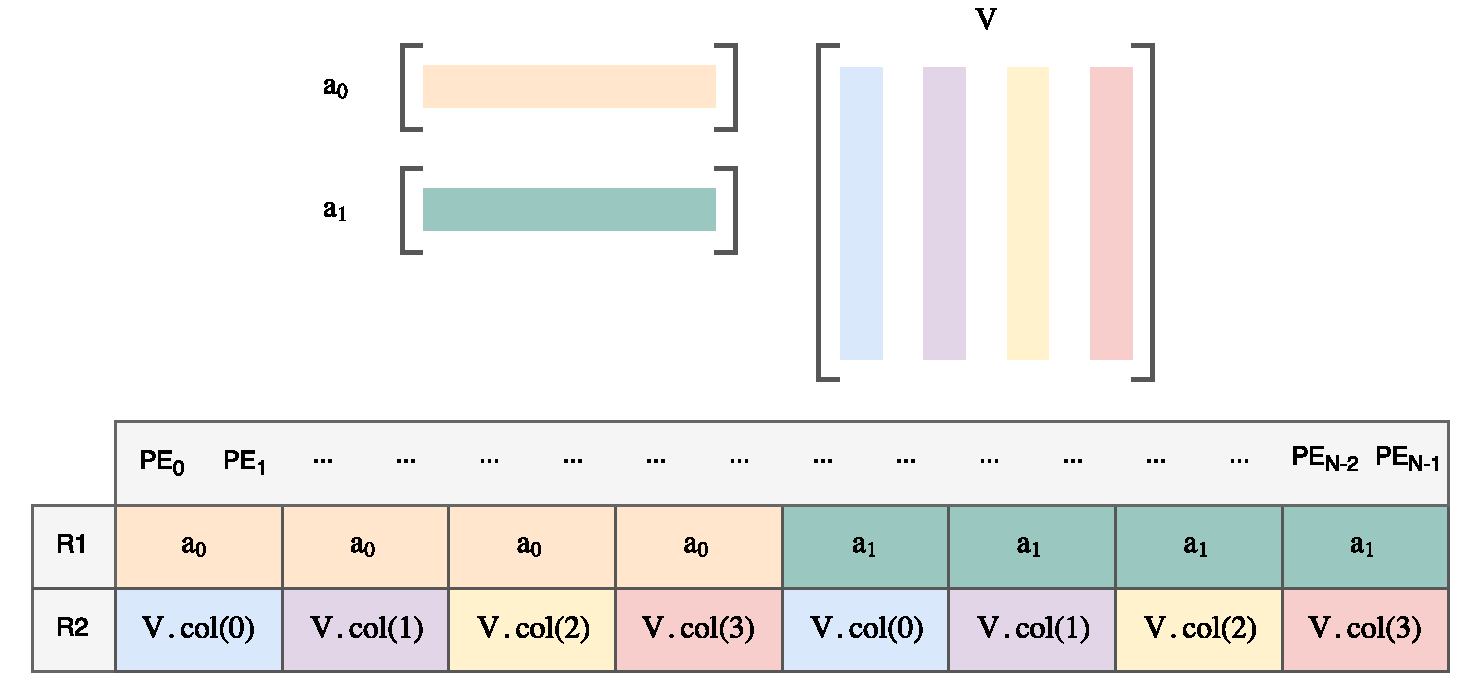
\includegraphics[width=0.7\textwidth]{src/img/vec-matrix-more-mult}
    \caption{Exemplu de aranjare a elementelor în ConnexArray pentru o înmulțire
    dintre doi vectori și aceeași matrice}
    \label{fig:cnx-more-mult}
\end{figure}

Am dorit crearea unui kernel distinct pentru fiecare dintre cele trei
situații de mai sus, deoarece putem optimiza folosirea resurselor, fără
adăugarea unei întârzieri suplimentare la execuție, putând selecta, în funcție
de caz, kernelul dorit.

\lstset{
    language=C++,
    directivestyle={\color{black}},
    emph={int,char,double,float,unsigned},
    emphstyle={\color{RoyalBlue}}
}
\begin{lstlisting}[
    caption={Pseudocod pentru înmulțirea dintre un vector și o matrice atunci
    când cel puțin o matrice poate fi scrisă într-o linie din memoria locală},
    label={lst:pseudocode-mult-a}
]
for i = 1 to y:
  load input array from LS[i];
  multiply registers;
  for j = 1 to arr_size_c * k:
    select block to reduce;
    reduce;
\end{lstlisting}

\lstset{
    language=C++,
    directivestyle={\color{black}},
    emph={int,char,double,float,unsigned},
    emphstyle={\color{RoyalBlue}}
}
\begin{lstlisting}[
    caption={Pseudocod pentru înmulțirea dintre un vector și o matrice atunci
    când cel puțin o coloană poate fi scrisă într-o linie din memoria locală},
    label={lst:pseudocode-mult-b}
]
for i = 1 to y:
  load input array from LS[x+i-1];
  for j = 1 to x-1:
    load matrix block from LS[j-1];
    multiply registers;
    for jj = 1 to k:
      select block to reduce;
      reduce;

  load last matrix block from LS[x-1];
  multiply registers;
  for all partial blocks to reduce:
    select block to reduce;
    reduce block;
\end{lstlisting}

\lstset{
    language=C++,
    directivestyle={\color{black}},
    emph={int,char,double,float,unsigned},
    emphstyle={\color{RoyalBlue}}
}
\begin{lstlisting}[
    caption={Pseudocod pentru înmulțirea dintre un vector și o matrice atunci
    când o coloană din matrice ocupă mai multe linii din memoria locală},
    label={lst:pseudocode-mult-c}
]
for i = 1 to y:
  for ii = 1 to N:
    reset the array pointer ARR_PTR = x + (i-1) * n;
    for j = 1 to n:
      load current matrix block from LS[(j-1)*n];
      load current array chunk from LS[ARR_PTR];
      multiply registers;
      reduce processing line;
      ARR_PTR++;
    ARR_PTR++;
\end{lstlisting}

\begin{figure}[h]
\centering
\captionsetup{justification=centering}
\subfloat[Cazul în care o linie din LS conține cel puțin o matrice (sistem cu 2 - 8 antene).]{
  \label{fig:chunking-a}
  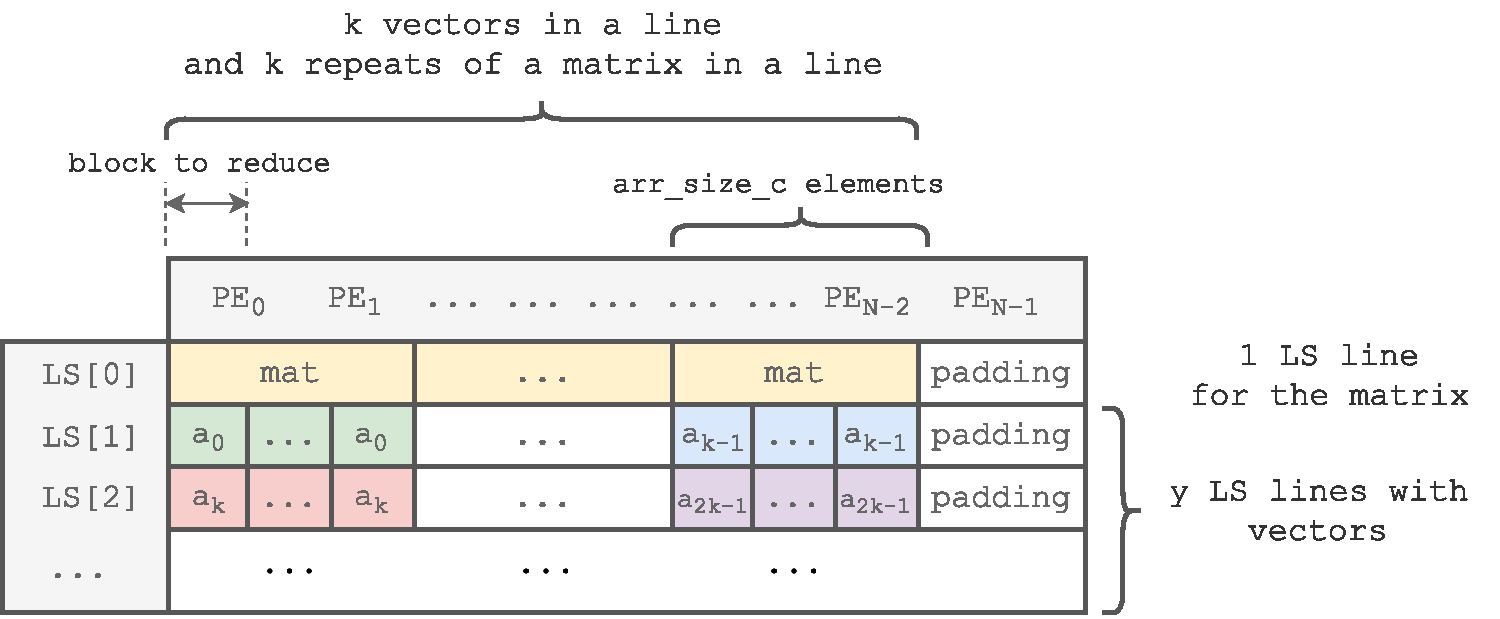
\includegraphics[scale=.5]{src/img/chunking-mult-a}}
  \phantomcaption
\end{figure}
~
\begin{figure}[h]\ContinuedFloat
\centering
\captionsetup{justification=centering}
\subfloat[Cazul în care o linie din LS conține cel puțin o coloană din matricea de
intrare (sistem cu 9 - 64 antene).]{
  \label{fig:chunking-b}
  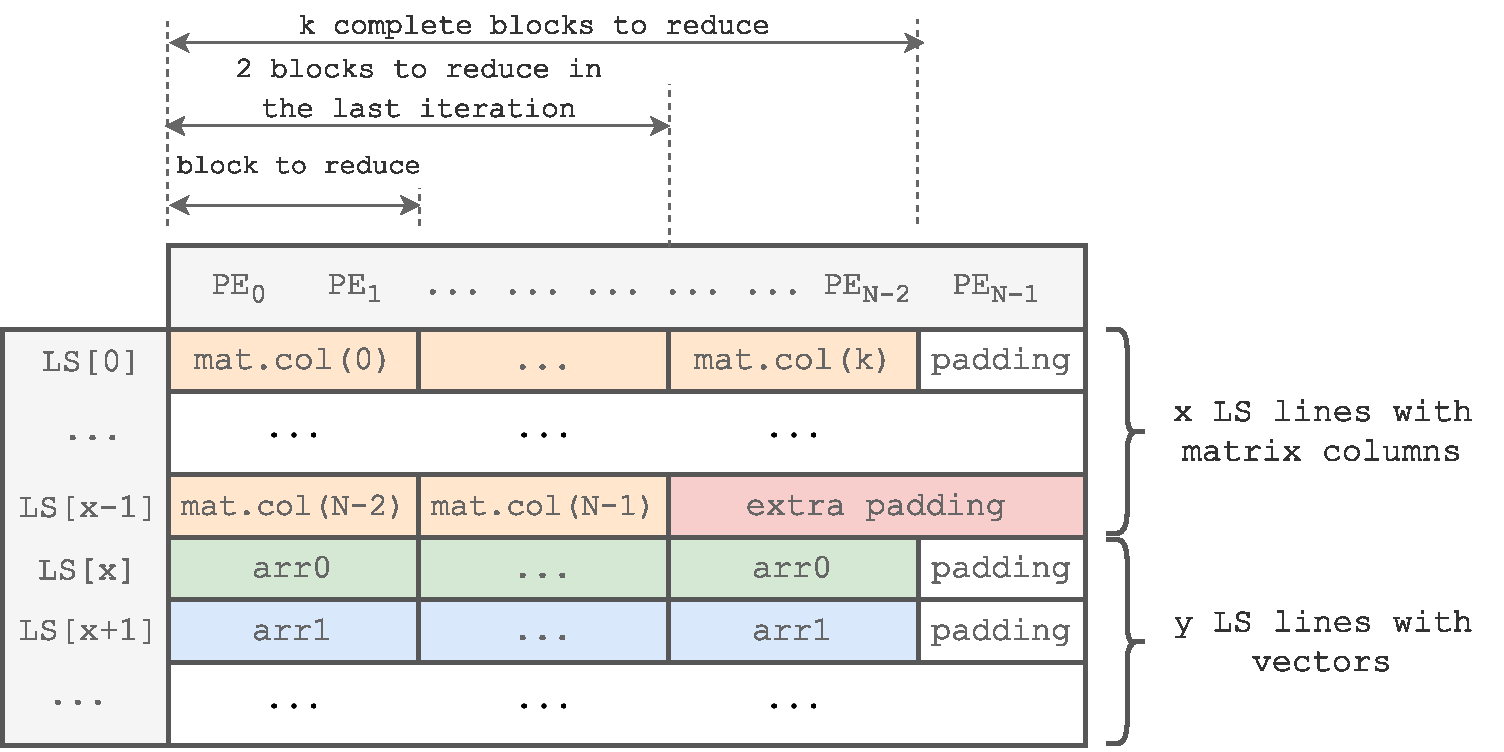
\includegraphics[scale=.5]{src/img/chunking-mult-b}}
  \phantomcaption
\end{figure}
~
\begin{figure}[h]\ContinuedFloat
\centering
\captionsetup{justification=centering}
\subfloat[Cazul în care o coloană dintr-o matrice este stocată pe mai multe linii din
LS (sistem cu mai mult de 64 antene).]{
  \label{fig:chunking-c}
  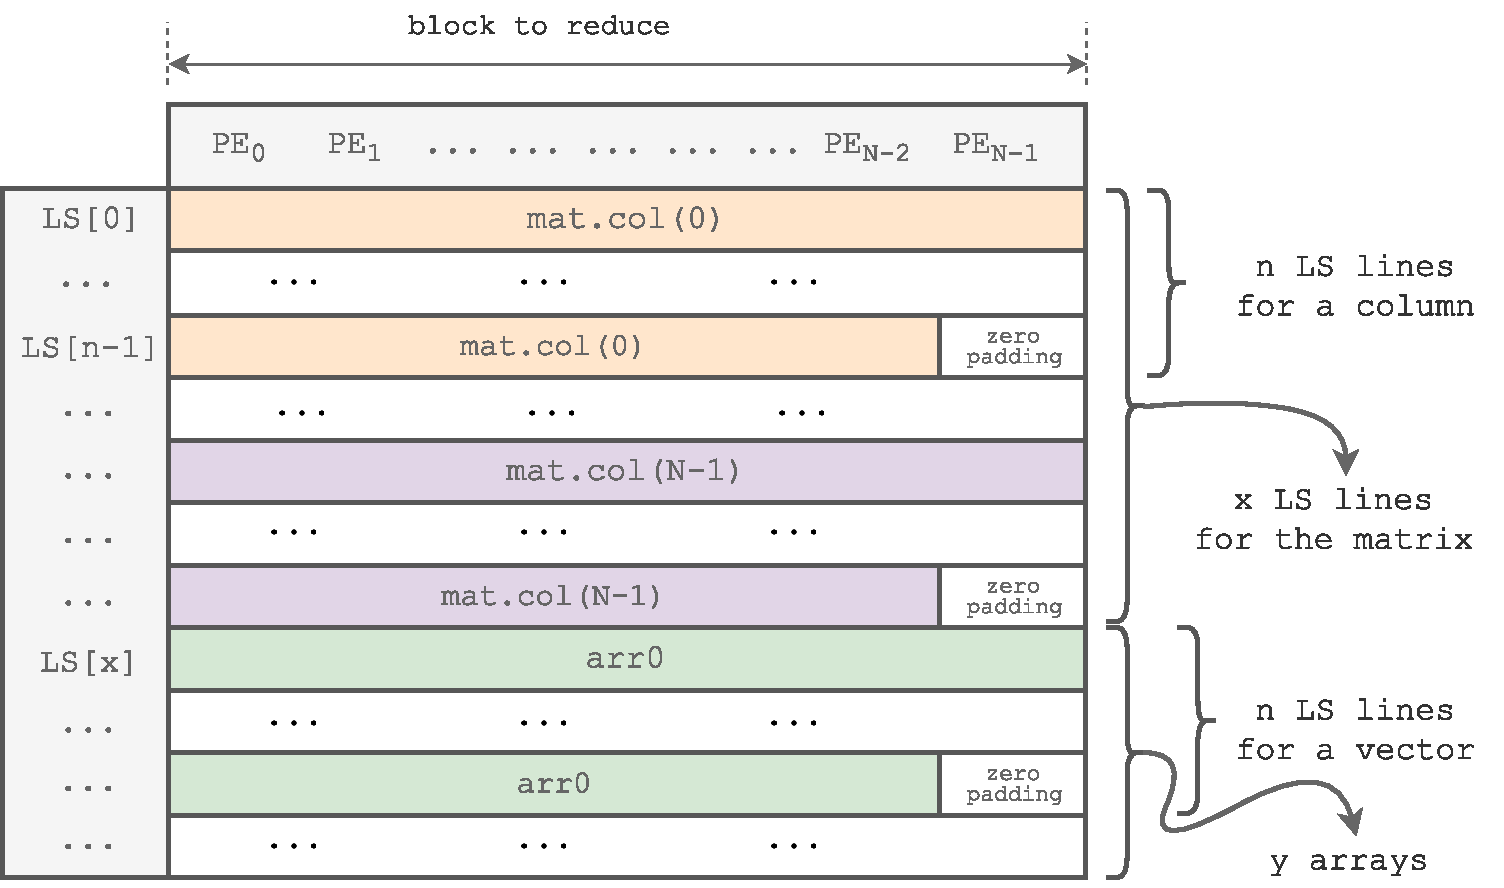
\includegraphics[scale=.5]{src/img/chunking-mult-c}}
\caption{Organizarea elementelor în memoria locală a acceleratorului în cazul
înmulțirii dintre un vector linie și o matrice.}
\label{fig:chunking-main}
\end{figure}

%=============================================================================
% KERNEL VECTOR x MATRICE x VECTOR
%=============================================================================
\section{Kernel pentru produsul înlănțuit dintre un vector linie, o matrice
pătratică și un vector coloană}
\label{sec:kernel-mult-chain}

În secțiunea precedentă a fost descris un algoritm pentru realizarea înmulțirii
dintre un vector linie și o matrice pătratică, adică prima parte a înmulțirii de
la numitorul Ecuației \eqref{eq:music-spectrum-kernel}, notată 
$X_M \overset{\Delta}{=} \bm{a}^H(\theta)\bm{V}_{N_{sq}}$. Dorim acum să găsim un
algoritm pentru a realiza întregul produs
$\bm{a}^H(\theta)\bm{V}_{N_{sq}}\bm{a}(\theta)$.  Elaborând pe baza relațiilor
obținute anterior, avem:
\begin{equation}
  X_M\bm{a}(\theta)
  =
  \begin{bmatrix}
    \displaystyle{\sum_{i=0}^{M-1} \overline{a_i}v_{i,0}} & 
    \displaystyle{\sum_{i=0}^{M-1} \overline{a_i}v_{i,1}} & 
    \hdots &
    \displaystyle{\sum_{i=0}^{M-1} \overline{a_i}v_{i,M-1}}
  \end{bmatrix}
  \begin{bmatrix}
    a_0   \\   
    a_1   \\   
    \vdots   \\   
    a_{M-1}
  \end{bmatrix}
\end{equation}
Deducem că întregul produs se poate scrie și sub forma:
\begin{equation}
  P_{MUSIC}(\theta)^{-1}
  =
  \begin{bmatrix}
    \displaystyle{a_0\sum_{i=0}^{M-1} \overline{a_i}v_{i,0}} +
    \displaystyle{a_1\sum_{i=0}^{M-1} \overline{a_i}v_{i,1}} +
    \hdots +
    \displaystyle{a_{M-1}\sum_{i=0}^{M-1} \overline{a_i}v_{i,M-1}}
  \end{bmatrix}
\end{equation}
Putem scrie una din sumele de produse sub forma: \\
\begin{equation}
  a_k\sum_{i=0}^{M-1} \overline{a_i}v_{i,k} = 
  a_k\Bigg(
       \sum_{i=0}^{M-1} (x_ix_{i,k} - \overline{y}_iy_{i,k}) + 
      j\sum_{i=0}^{M-1}(x_iy_{i,k} + \overline{y}_ix_{i,k})
      \Bigg)
\end{equation}
Notăm
\begin{equation}
  E_{i,k}^{(1)} \overset{not}{=} x_ix_{i,k} - \overline{y}_iy_{i,k}, \quad 
  i = \overline{0, M-1}, k = \overline{0, M-1}
\end{equation}
\begin{equation}
  E_{i,k}^{(2)} \overset{not}{=} x_iy_{i,k} + \overline{y}_ix_{i,k}, \quad
  i = \overline{0, M-1}, k = \overline{0, M-1}
\end{equation}
și putem scrie:
\begin{equation}
  a_k\sum_{i=0}^{M-1} \overline{a_i}v_{i,k} = 
  (x_k + jy_k)
  \Bigg(
  \sum_{i=0}^{M-1} E_{i,k}^{(1)}+ j\sum_{i=0}^{M-1} E_{i,k}^{(2)}
  \Bigg)
\end{equation}
\begin{equation}
  a_k\sum_{i=0}^{M-1} \overline{a_i}v_{i,k} = 
  \Bigg(
  x_k \sum_{i=0}^{M-1} E_{i,k}^{(1)} - y_k \sum_{i=0}^{M-1} E_{i,k}^{(2)}
  \Bigg) + 
 j\Bigg(
  x_k \sum_{i=0}^{M-1} E_{i,k}^{(2)} + y_k \sum_{i=0}^{M-1} E_{i,k}^{(1)}
  \Bigg)
\end{equation} 
% Notăm produsele componente ale expresiilor E1 și E2:
% \begin{equation}
%   re_{i,k}^{(1)} \overset{not}{=} x_ix_{i,k}, \quad 
%   re_{i,k}^{(2)} \overset{not}{=} \overline{y}_iy_{i,k}, \quad 
%   i = \overline{0, M-1}, k = \overline{0, M-1}
% \end{equation}
% și, respectiv,
% \begin{equation}
%   im_{i,k}^{(1)} \overset{not}{=} x_iy_{i,k}, \quad 
%   im_{i,k}^{(2)} \overset{not}{=} \overline{y}_ix_{i,k}, \quad
%   i = \overline{0, M-1}, k = \overline{0, M-1}
% \end{equation} \\

În Secțiunea~\ref{sec:kernel-mult}, unde am detaliat înmulțirea a doi vectori de
numere complexe, am considerat aranjamentul datelor din
registrele acceleratorului din Figura \ref{fig:complex-mult}, iar cu notațiile
făcute observăm că produsele componente ale expresiei $E_{i,k}^{(1)}$ se găsesc
în registrele R3, iar produsele componente ale expresiei $E_{i,k}^{(2)}$ au fost
reținute în registrele R4, unde $k = \overline{0, M-1}$ reprezintă coloana din
matricea $\bm{V}_N{_{sq}}$ pentru care au fost calculate. Rezultă că, dacă
înmulțim partea reală a unui element $a_k$ din vectorul $a(\theta)$ cu fiecare
produs component al expresiei $E_{i,k}^{(1)}$ corespunzătoare unei coloane $k$
și, similar, partea imaginară (cu semn schimbat) a aceluiași element cu fiecare
produs din expresia $E_{i,k}^{(2)}$ și sumăm produsele astfel obținute din toate
coloanele, vom obține o valoare a spectrului MUSIC. \\

\begin{figure}[h]
    \centering
    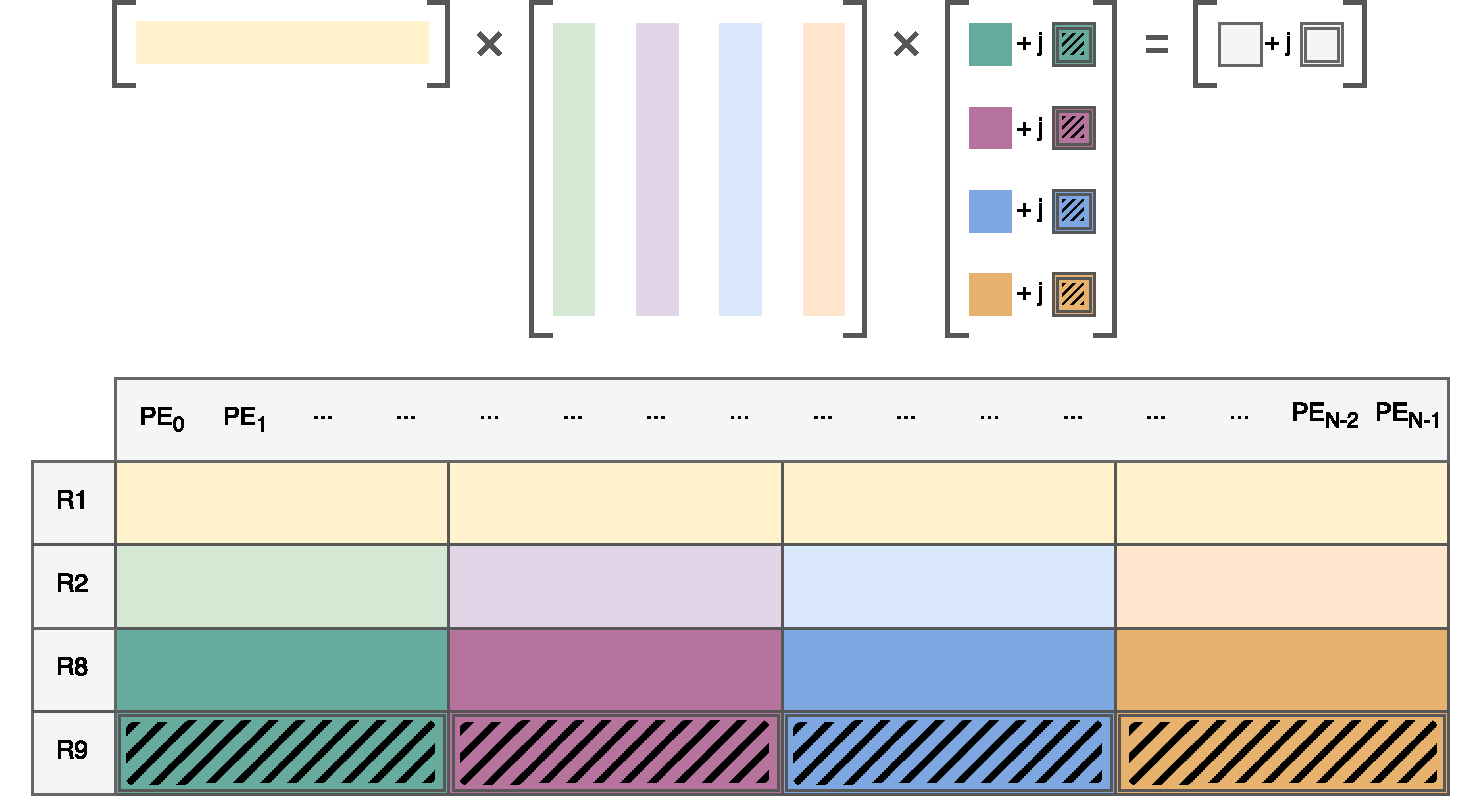
\includegraphics[width=0.8\textwidth]{src/img/mult-chained}
    \caption{Aranjarea elementelor vectorilor în ConnexArray în cazul înmulțirii
    înlănțuite a unui vector, o matrice și a altui vector}
    \label{fig:reg-mult-chain}
\end{figure}

Aranjamentul propus, particularizat pentru doi vectori de lungime egală cu 4 și
o matrice pătratică de dimensiune $4 \times 4$, este ilustrat în figura
\ref{fig:reg-mult-chain}. Partea imaginară a unui număr este marcată printr-o
figură hașurată și se observă cum părțile reale și imaginare sunt
repetate pe lungimea unei coloane a matricei pentru a putea fi obținute
produsele anterior menționate. \\

În cazul unor serii de astfel de înmulțiri înlănțuite care folosesc aceeași
matrice de intrare (cum este cazul în algoritmul MUSIC), aranjarea elementelor
vectorilor se va face în mod similar cu cazul înmulțirii dintre un vector linie
și o matrice din Figura \ref{fig:chunking-main}, modificarea constând în faptul că
în memorie vom avea trei zone: una pentru elementele
vectorului linie, una pentru părțile reale ale vectorului coloană și una pentru
părțile imaginare ale acestuia. Prin urmare, un dezavantaj al acestei metode va
consta în faptul că vom putea cuprinde mai puține elemente de intrare
într-o execuție decât în cazul precedent. \\ 

În cazul în care \code{mat\_size\_c} $\le$ \code{vector\_array\_size}, cele trei
zone de memorie vor fi egale. Dacă, însă, \code{mat\_size\_c} $>$
\code{vector\_array\_size}, fiecare vector linie va trebui stocat o singură
dată, dar elementele vectorului coloană vor ocupa un număr egal de linii din LS
ca și matricea de intrare. În Anexa \ref{sec:kernel-mult-chained} se găsește
implementarea kernelului pentru prima situație descrisă și o comparație între
cele două metode va fi realizată în Capitolul \ref{chapter:eval}, Secțiunea
\ref{sec:eval-music}.


% 
% \begin{figure}[H]
% \centering
% \captionsetup{justification=centering}
% \subfloat[Cazul în care o linie din LS conține cel puțin o matrice (sistem cu 2 - 8 antene).]{
%   \label{fig:chunking-chained-a}
%   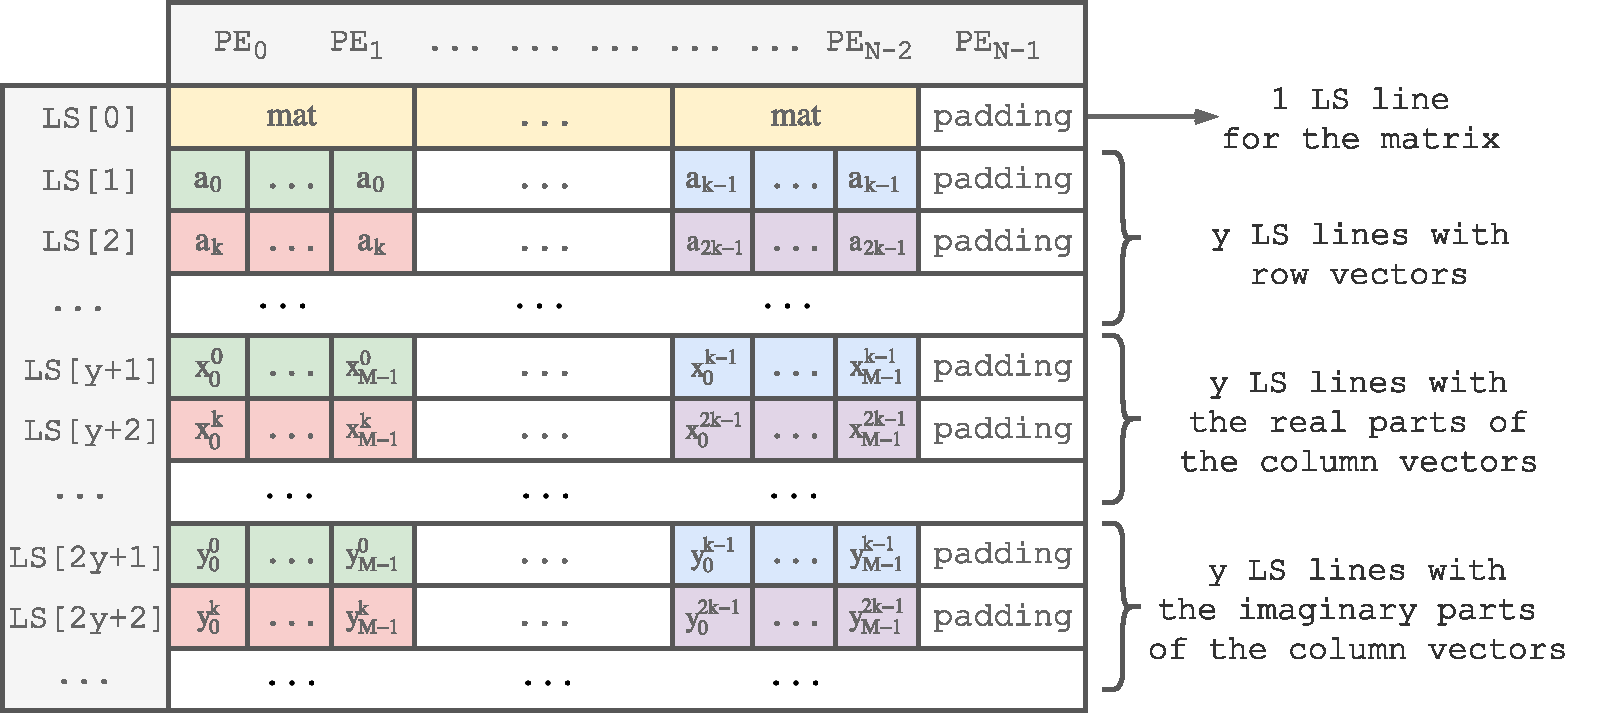
\includegraphics[scale=.5]{src/img/chunking-chained-a}}
% \end{figure}
% ~
% \begin{figure}[h]\ContinuedFloat
% \centering
% \captionsetup{justification=centering}
% \subfloat[Cazul în care o linie din LS conține cel puțin o coloană din matricea de
% intrare (sistem cu 9 - 64 antene).]{
%   \label{fig:chunking-chained-b}
%   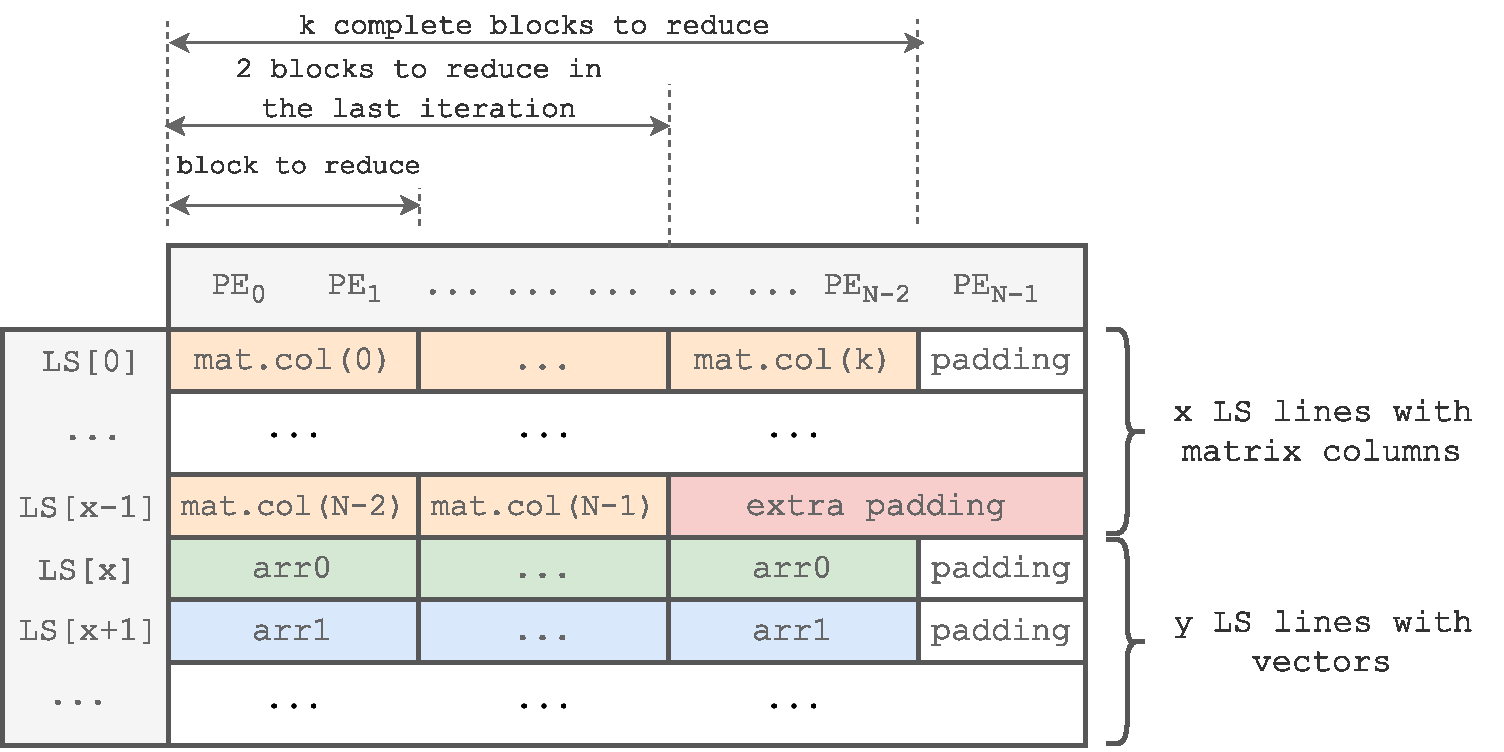
\includegraphics[scale=.5]{src/img/chunking-chained-b}}
% \end{figure}
% ~
% \begin{figure}[h]\ContinuedFloat
% \centering
% \captionsetup{justification=centering}
% \subfloat[Cazul în care o coloană dintr-o matrice este stocată pe mai multe linii din
% LS (sistem cu mai mult de 64 antene).]{
%   \label{fig:chunking-chained-c}
%   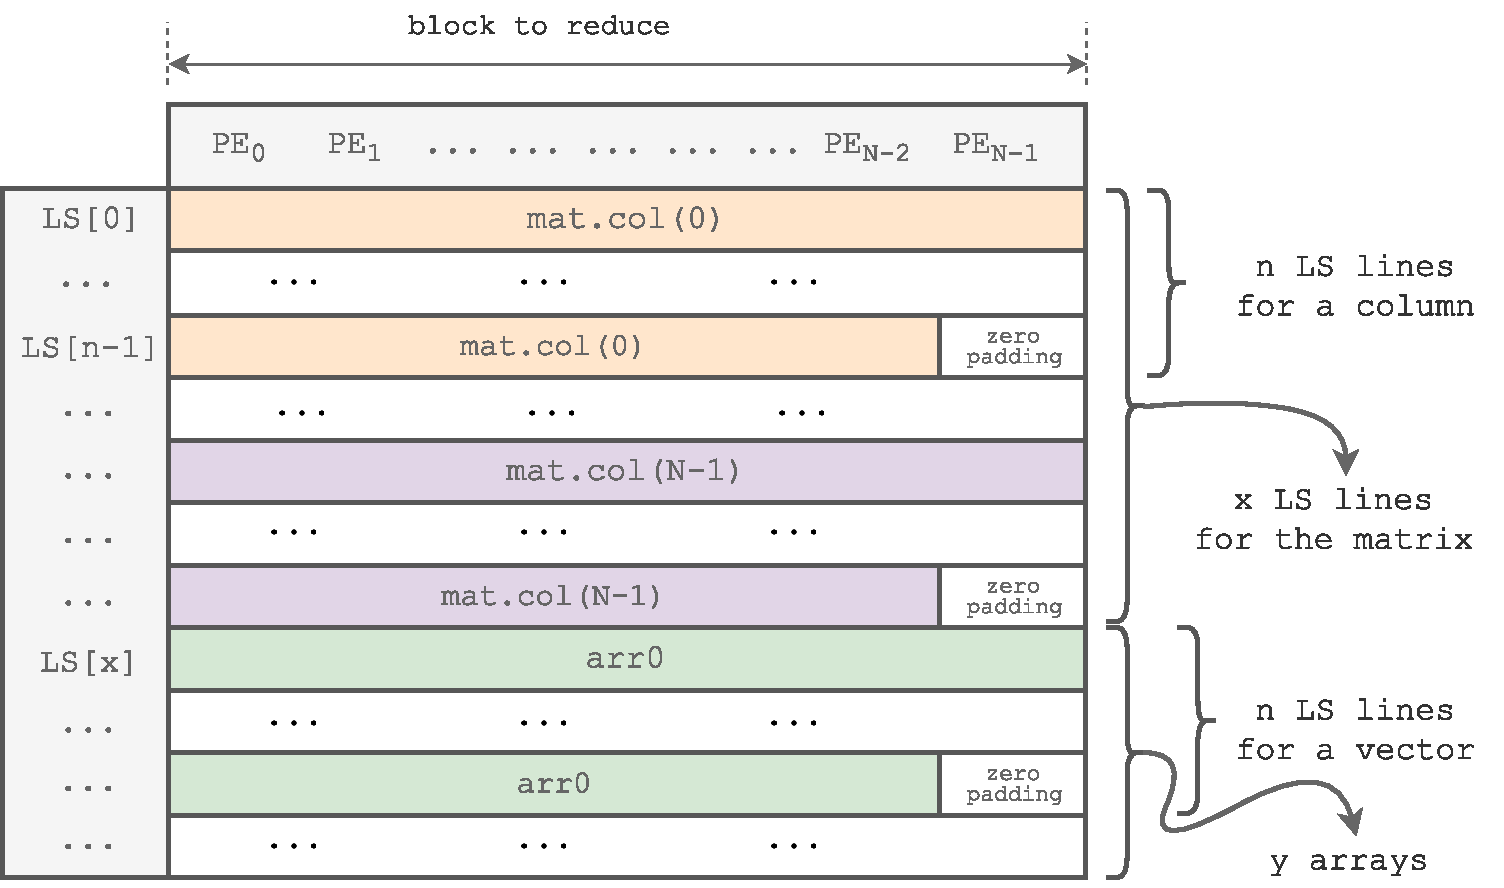
\includegraphics[scale=.5]{src/img/chunking-chained-c}}
% \caption{Organizarea elementelor în memoria locală a acceleratorului în cazul
% înmulțirii dintre un vector linie și o matrice.}
% \label{fig:chunking-main}
% \end{figure}


%=============================================================================
% KERNEL AUTOCORELAȚIE SEMNAL
%=============================================================================

\section{Kernel pentru autocorelația unui semnal}
\label{sec:kernel-autocorr}

Metoda de realizare a autocorelației a fost descrisă în
Secțiunea~\ref{ssec:autocorrelate-block}, conceptul de bază fiind faptul că
autocorelația este estimată prin intermediul eșantioanelor semnalului de intrare
care ajunge la cele N antene, efectuată pe o ,,captură'' de K eșantioane. Ca pas
opțional, se poate aplica și o mediere antegradă-retrogradă pentru o acuratețe
mai bună a estimării. \\

Primul pas este estimarea matricei de autocorelație $\bm{C}_X$ din matricea
formată din cele K eșantioane de la cele N semnale de intrare:
\begin{equation}
\bm{C}_X = \frac{1}{K}\bm{X}\bm{X}^H.
\end{equation}

Estimatul matricei de autocorelație devine:
\begin{equation}
    \bm{X}
    \overset{\Delta}{=}
    \begin{bmatrix}
        x_{0,0}   &   x_{0,1}   &   \hdots   &   x_{0,K-1} \\
        x_{1,0}   &   x_{1,1}   &   \hdots   &   x_{1,K-1} \\
        \vdots    &   \vdots    &   \ddots   &   \vdots    \\
        x_{N-1,0} &   x_{N-1,1} &   \hdots   &   x_{N-1,K-1}
    \end{bmatrix}
\end{equation}

\begin{equation}
    \bm{C}_X
    = \bm{X} \bm{X}^H = 
    \begin{bmatrix}
        \displaystyle{\sum_{n=\overline{0, K-1}} x_{0,n}x_{n,0}^*} & 
        \displaystyle{\sum_{n=\overline{0, K-1}} x_{0,n}x_{n,1}^*} & 
        \hdots &
        \displaystyle{\sum_{n=\overline{0, K-1}} x_{0,n}x_{n,N-1}^*} \\
        \displaystyle{\sum_{n=\overline{0, K-1}} x_{1,n}x_{n,0}^*} & 
        \displaystyle{\sum_{n=\overline{0, K-1}} x_{1,n}x_{n,1}^*} & 
        \hdots &
        \displaystyle{\sum_{n=\overline{0, K-1}} x_{1,n}x_{n,N-1}^*} \\
        \vdots & \vdots & \ddots & \vdots \\
        \displaystyle{\sum_{n=\overline{0, K-1}} x_{N-1,n}x_{n,0}^*} & 
        \displaystyle{\sum_{n=\overline{0, K-1}} x_{N-1,n}x_{n,1}^*} & 
        \hdots &
        \displaystyle{\sum_{n=\overline{0, K-1}} x_{N-1,n}x_{n,N-1}^*}
    \end{bmatrix}
\end{equation}
unde
\begin{equation}
x_{m,n} = a_{m,n} + jb_{m,n}, \quad m = \overline{0, M-1}, n = \overline{0, M-1}
\end{equation}

Deci, un element $c_{m, n}$ al matricei $\bm{C}_X$ este:
\begin{equation}
c_{m, n} = \displaystyle{
           \sum_{k=0}^{K-1} (a_{m,k}a_{k,n} + b_{m,k}b_{k,n}) + 
          j\sum_{k=0}^{K-1} (-a_{m,k}b_{k,n} + b_{m,k}a_{k,n})}
\end{equation}

Observăm că $\bm{C}_X$ este o matrice Hermitică, deci $c_{ij} =
\overline{c_{ji}}$, unde $c_{ij}$ este un element al matricei și  $i =
\overline{0, N-1}$, $j = \overline{0, N-1}$, ceea ce înseamnă că va fi de ajuns
să calculăm doar elementele de pe diagonala principală și de deasupra ei. \\

În plus, se observă că expresia unui element de-al matricei de autocorelației
este foarte asemnănătoare cu cea obținută în Ecuația
\eqref{eq:expresie-inmultire}, deci algoritmul precedent va putea fi aplicat cu
modificări minime. \\

\begin{figure}[h]
    \centering
    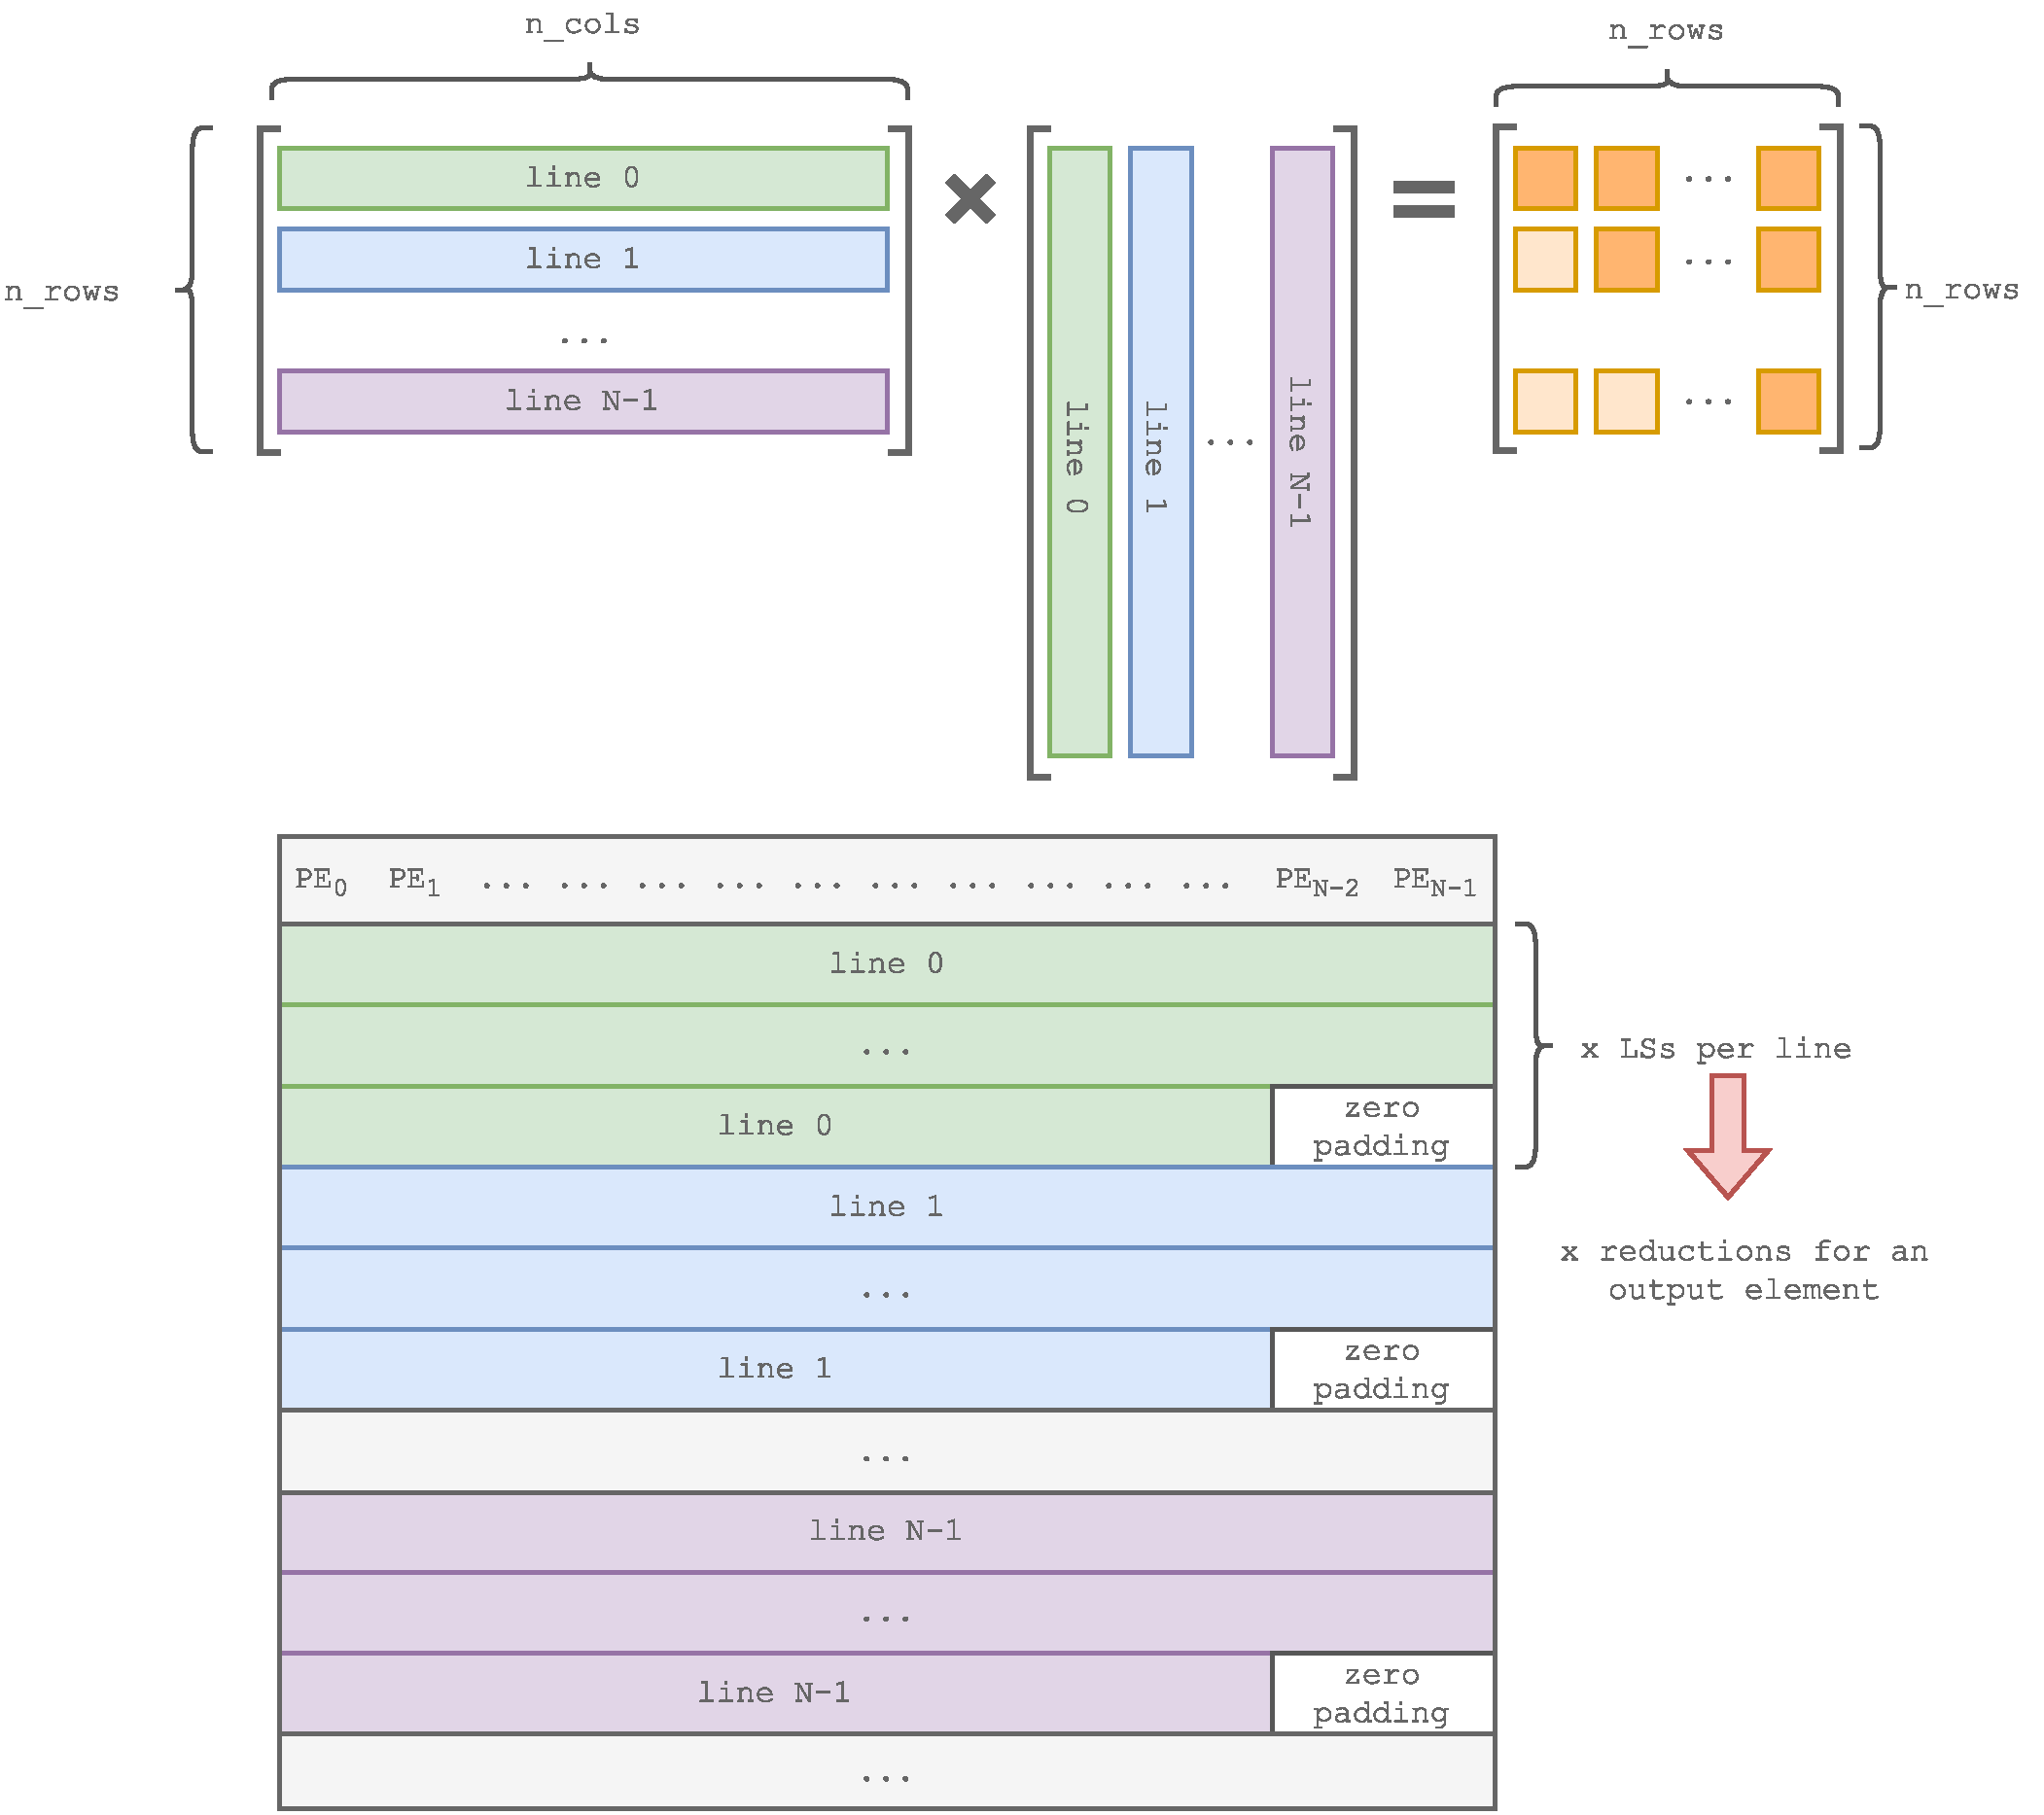
\includegraphics[width=1\textwidth]{src/img/autocorrelation}
    \caption{Aranjarea datelor de intrare în acceleratorul ConnexArray pentru un
    kernel care calculează autocorelația unui semnal}
    \label{fig:autocorrelation-in-ls}
\end{figure}

Dorim să avem în fiecare execuție a kernelului un număr cât mai mare de date de
procesat, prin urmare, vom încerca să realizăm întreaga înmulțire de matrice
într-o singură execuție. Deși autocorelația se realizează între o matrice și
hermitica ei, vom prefera să încărcăm doar matricea de intrare în forma inițială
în memoria acceleratorului, precum în Figura \ref{fig:autocorrelation-in-ls} și
să adaptăm calculul înmulțirii, astfel încât nu se mai inversează semnul
produselor $b_{m,k}b_{k,n}$, ci semnul produselor de forma $a_{m,k}b_{k,n}$,
unde $k = \overline{0, K-1}$. Listarea \ref{lst:autocorr-kernel-pseudocode}
conține un pseudocod pentru modul de lucru descris pentru kernel, iar în
Anexa \ref{sec:kernel-autocorr-code} se găsește și implementarea acestuia.\\ 

\begin{lstlisting}[
    caption={Pseudocod pentru kernel care realizează autocorelația unui semnal},
    label={lst:autocorr-kernel-pseudocode}
]
for i = 1 to N
  load LS[i];
  for j = i to N
    load LS[j];
    multiply registers and invert signs;
    reduce registers;
\end{lstlisting}

În cazul de față, memoria locală are o capacitate de $1024 \cdot 128$ elemente
de 16 biți, iar numărul de elemente necesare pentru a încărca matricea este $2
\cdot N \cdot K$, deoarece părțile reale și cele imaginare ale datelor de
intrare sunt considerate elemente distincte. Prin urmare, avem o flexibilitate
destul de mare în alegerea configurației sistemului. Pentru un sistem ce conține
64 antene, de exemplu, putem avea o dimensiune maximă a capturii de 1024
elemente, care oferă o acuratețe satisfăcătoare a rezultatului final de aproximativ
$0.15^{\circ}$. Dacă se dorește folosirea unui număr mai mare de antene și o
estimare mai imprecisă a autocorelației nu este acceptabilă, procesarea poate
fi, și în acest caz, împărțită în blocuri de procesare egale, încărcând liniile
necesare astfel încât să obținem toate produsele dorite.

%=============================================================================
% INTEGRARE GNU RADIO
%=============================================================================
\section{Integrarea kernelurilor in GNU Radio}
\label{sec:kernel-integrate}

Întrucât kernelurile au o funcționalitate generică, putând fi folosite și pentru
alți alogritmi de procesare de semnale, am dorit integrarea lor în blocuri
dintr-un modul OOT în GNU Radio, pentru a fi independente de lanțul de procesare
pentru algoritmul MUSIC ales. \\

Este important de avut în vedere faptul că blocurile vor trebui să comunice cu
cozile acceleratorului, deci vor avea nevoie de căile către acestea pentru a
putea crea o instanță a obiectului \code{ConnexMachine} dependentă de
acceleratorul folosit, pe care le vor primi ca parametri de intrare odată cu
crearea blocului. Programul principal, care instanțiază blocul, va primi, la
rândul său, aceste căi ca argumente în linia de comandă. Vom folosi un script
pentru lansarea sa în execuție, în care putem specifica dacă dorim să folosim
simulatorul sau echipamentul hardware, programul în sine fiind agnostic în
legătură cu acest aspect. Diferența va consta doar în căile primite ca argument.
În continuare, vor fi descrise specificațiile blocurilor pentru fiecare kernel
creat.

\subsection{Bloc GNU Radio pentru realizarea înmulțirii dintre o serie de
vectori linie și o matrice}

Deoarece cazul în care vom avea de înmulțit un singur vector linie cu o singură
matrice este simplu de efectuat și deoarece există situații în care va fi necesar să
calculăm produsul dintre mai mulți vectori și aceeași matrice (cum este cazul în
algoritmul MUSIC), am preferat pentru implementare cea de-a doua variantă.

Am creat un bloc de sine stătător care are două
intrări și o ieșire de tip vectori de numere complexe, ceea ce înseamnă că
elementele nu sunt procesate unul câte unul, ci se așteaptă colectarea unui număr
suficient de elemente de intrare pentru a putea începe procesarea unui element
de ieșire, care este la rândul său de tip vector de numere complexe.
Specificațiile intrărilor și ieșirii sunt următoarele, ilustrate și în Figura
\ref{fig:multiply-cc}:
\begin{itemize}
  \item Prima intrare - primește blocuri de câte \code{nr\_arrays} vectori de
  lungime \code{arr\_size}, de tip de date complex.

  \item A doua intrare  - primește o matrice pătratică de dimensiune \code{arr\_size x
  arr\_size}, stocată în memorie coloană cu coloană.

  \item Ieșire - rezultatul înmulțirii dintre cele \code{nr\_arrays} vectori de
  intrare și matrice. Din moment ce rezultatul înmulțirii dintre un singur
  vector și o matrice conține \code{arr\_size} elemente, ieșirea va avea în
  total un număr de \code{arr\_size x nr\_arrays} elemente.
\end{itemize}

\begin{figure}[h]
    \centering
    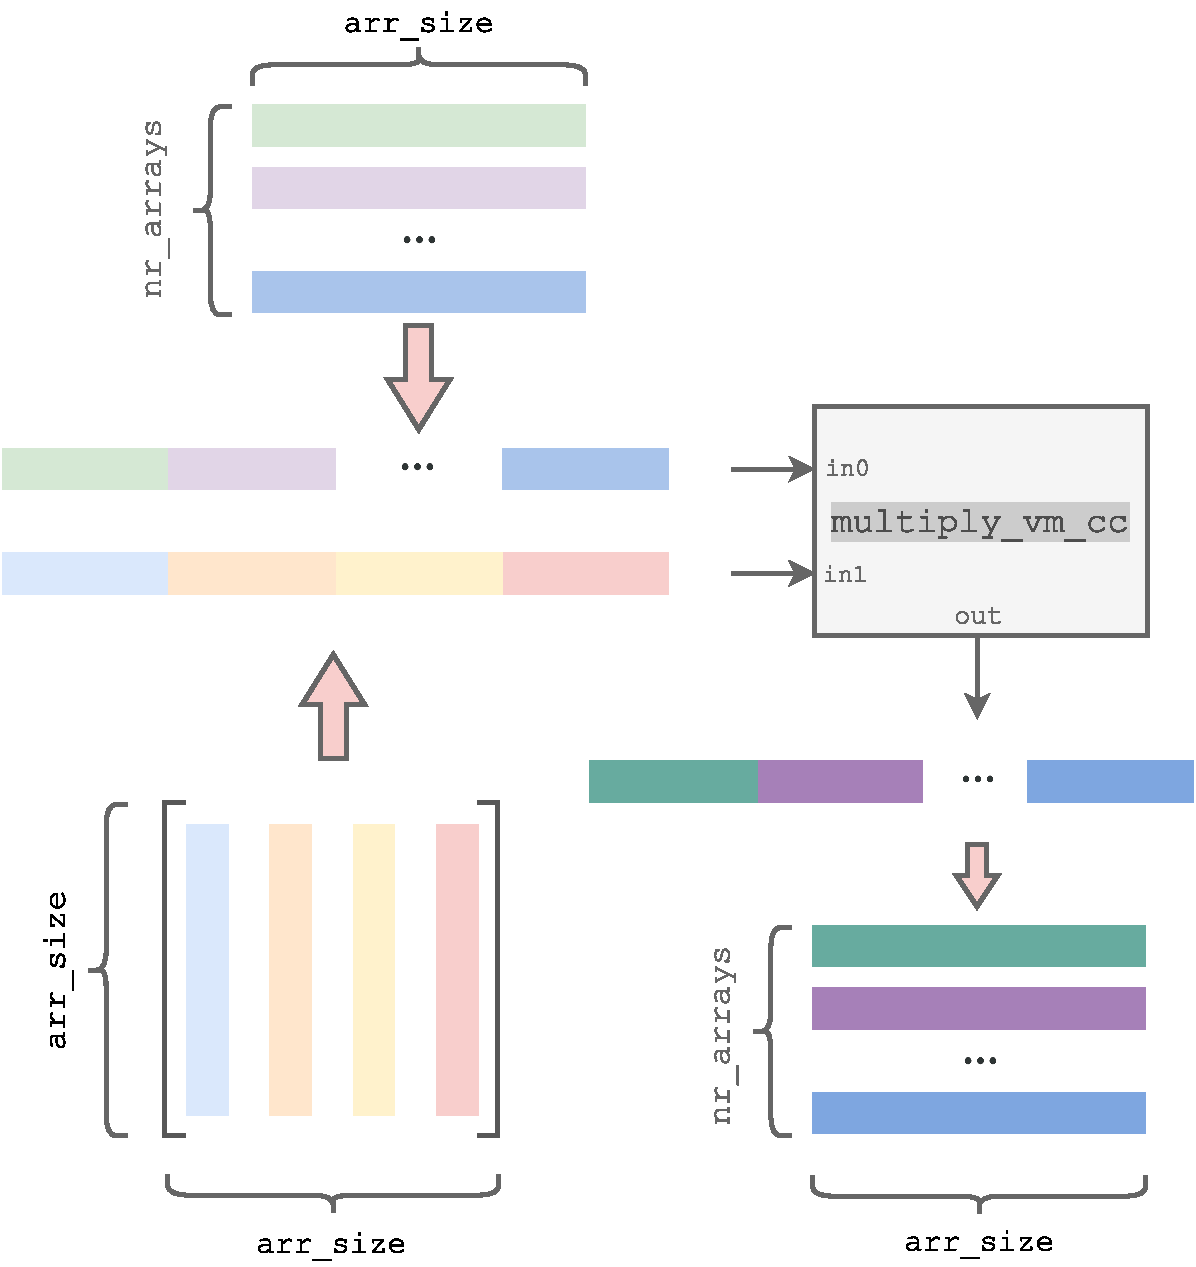
\includegraphics[width=0.7\textwidth]{src/img/multiply-cc}
    \caption{Structura intrărilor și ieșirilor blocului GNU Radio care
    realizează înmulțirea dintre o serie de vectori de intrare și aceeași
    matrice}
    \label{fig:multiply-cc}
\end{figure}

Deoarece există relații diferite între numărul de elemente de intrare și cele de
ieșire necesare, blocul va fi de tip \code{general} și va folosi o metodă
\code{forecast} pentru a le asigura. Întrucât acceleratorul
ConnexArray are o capacitate de \code{vector\_array\_size = 128} PE-uri și
numărul de vectori pe prima intrare poate fi destul de mare, vom separa
elementele de intrare în blocuri care vor fi procesate succesiv. \\

Înaintea fiecărei lansări în execuție a unui kernel, datele de intrare trebuie
să fie ,,pregătite'', adică scalate și salvate într-un vector de elemente de tip
întreg, fără semn, pe 16 biți. Matricea de intrare poate fi pregătită o singură dată
pentru fiecare element de ieșire, în timp ce pentru vectorii de intrare acest
lucru trebuie să se facă la începutul fiecărui bloc. \\

După ce avem datele de intrare pregătite, putem să lansăm în execuție kernelul,
operație care nu este blocantă, deci firul de execuție principal își continuă
parcursul. Obținem datele de ieșire prin citirea unui număr de elemente din
coada de reducție. Spre deosebire de lansarea în execuție, citirea datelor din
coadă \textit{este} blocantă, deoarece trebuie să avem certitudinea că citim
datele corecte. Odată ce ele sunt gata, trebuie scalate înapoi și convertite la
tipul de date complex cu părțile reală și imaginară în virgulă mobilă, folosit
pentru datele de ieșire. \\

Decizia în privința procesării care se va efectua în paralel va fi luată în
capitolul \ref{chapter:eval}, deoarece trebuie să realizăm un profil al
programului pentru a stabili care sunt punctele critice ale programului ce ar
putea beneficia de un mod de lucru distribuit.

\subsection{Bloc GNU Radio pentru calcularea spectrului MUSIC}

În calculul spectrului MUSIC intervine, la numitorul acestuia, o înmulțire
înlănțuită dintre un vector linie, o matrice pătratică și un vector coloană
(transpusul și conjugatul vectorului linie) care, după cum a fost deja
menționat, lasă deschise cel puțin două moduri de abordare: fie vom realiza
prima parte a înmulțirii, cea dintre un vector linie și o matrice pătratică, pe
acceleratorul ConnexArray, iar rezultatul va fi înmulțit cu ultimul vector
coloană pe procesorul gazdă ARM, fie vom realiza întreaga înmulțire pe
procesorul ConnexArray. \\

În ambele cazuri, blocul GNU Radio pentru calcularea spectrului MUSIC primește
la intrare o matrice pătratică vectorizată ce reprezintă estimatul
autocorelației semnalului de intrare, care va fi descompus în vectori proprii ce
vor interveni în calculul spectrului MUSIC. În continuare, procesarea se face în
mod similar cu cea a blocului descris anterior, împărțind datele de intrare în
blocuri de procesare a căror dimensiune va fi stabilită în funcție de metoda
folosită, astfel încât memoria să fie ocupată la capacitate maximă într-o
execuție. Diferența va consta în faptul că vectorii care apar în înmulțire pot
fi pregătiți pentru procesarea pe accelerator o singură dată, în constructorul
blocului, eliminând, astfel, o parte importantă din punct de vedere
computațional. Matricea va fi pregătită pentru fiecare element de ieșire, ea
fiind comună tuturor înmulțirilor pentru un calcul al spectrului MUSIC. \\

În testarea acestui modul, au fost observate câteva aspecte important de
menționat:
\begin{itemize}
  \item În cazul primei variante, în care doar prima înmulțire dintre un vector
  linie și o matrice este realizată pe accelerator, am constatat că obținem o
  precizie medie a rezultatelor la ieșirea din accelerator de ordinul $10^{-4}$.
  În punctele spectrului MUSIC corespunzătoare unghiului de incidență al
  semnalului căutat, în teorie, numitorul expresiei spectrului ar trebui să fie
  cât mai apropiat de zero, iar spectrul MUSIC să aibă o valoare cât mai mare.
  În practică, acestea au valori de aproximativ $10^{-5} - 10^{-6}$ sau poate
  chiar mai mici, iar
  valorile din rezultatul înmulțirii intermediare sunt de ordinul $10^{-4} -
  10^{-5}$, dar din cauza faptului că precizia obținută cu folosirea datelor în
  virgulă fixă pe accelerator este de aproximativ $10^{-4}$, erorile în punctele
  de interes vor fi semnificative. Acest lucru conduce, în unele cazuri, la
  apariția mai multor maxime foarte apropiate în jurul unuia dintre unghiuri,
  care vor fi alese ambele drept unghiuri de incidență, în detrimentul unuia
  dintre unghiurile de incidență corecte. În Figura \ref{fig:correct-angles}
  este redată reprezentarea corectă a spectrului MUSIC, iar în Figura
  \ref{fig:incorrect-angles} este prezentată situația incorectă cauzată de
  precizia insuficientă. O soluție în acest sens ar fi modificarea algoritmului
  de căutare a maximelor locale ale spectrului MUSIC, astfel încât să ignore două puncte foarte
  apropiate și să caute altul, dacă acesta există. Acest lucru nu ar afecta
  neapărat rezoluția algoritmului, deoarece el nu poate distinge oricum între
  două surse de semnal foarte apropiate, dar va introduce o procesare în plus în
  blocul de căutare.

\begin{figure}[h]
\centering
\begin{minipage}{.5\linewidth}
  \subfloat[]{\label{fig:correct-angles}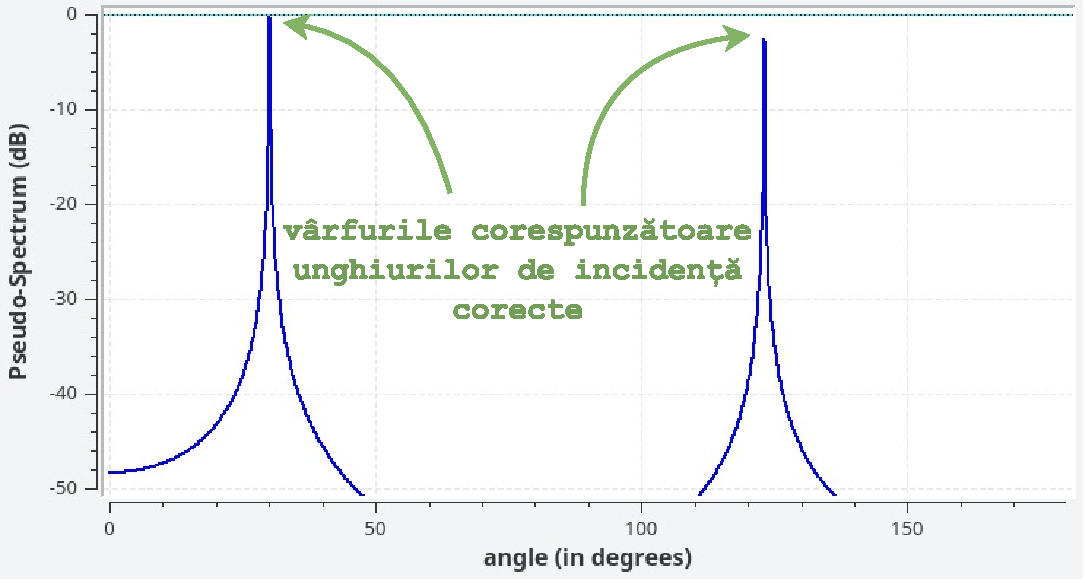
\includegraphics[scale=.45]{src/img/correct-angles-pdf}}
\end{minipage}%
\centering
\begin{minipage}{.5\linewidth}
  \subfloat[]{\label{fig:incorrect-angles}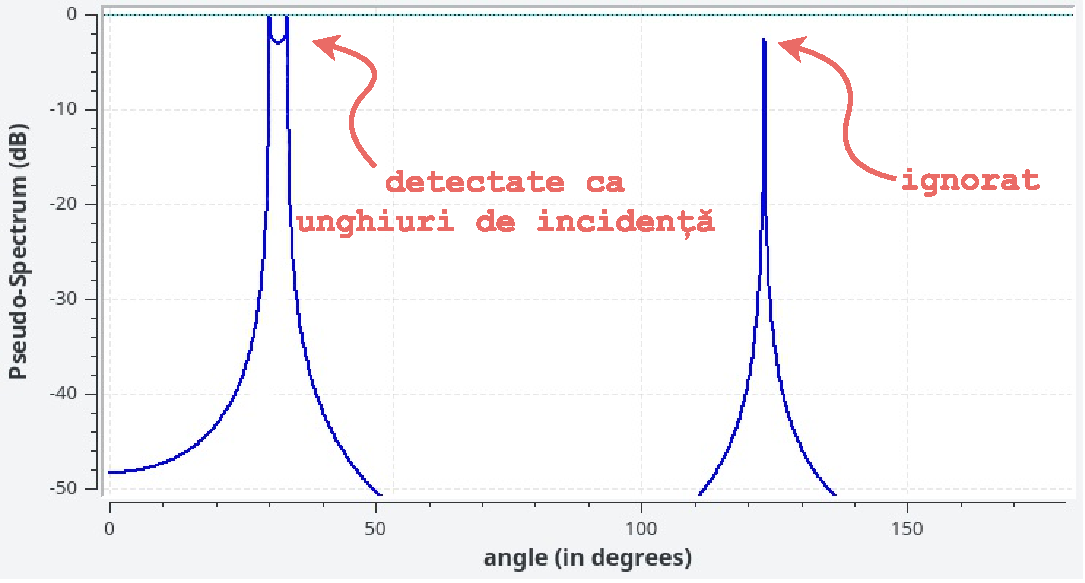
\includegraphics[scale=.45]{src/img/incorrect-angles-pdf}}
\end{minipage}\par\medskip

\caption{Reprezentările corectă și incorectă ale spectrului MUSIC}
\end{figure}


  \item În cazul în care folosim înmulțirea înlănțuită executată integral pe
  accelerator, datele vor avea de suferit, din nou, din cauza preciziei. Din
  cauza faptului că ultima înmulțire este realizată, și ea, pe accelerator,
  rezultatele cu ordin mai mic de $10^{-7} - 10^{-8}$ vor fi direct aproximate
  cu zero, ce conduce la o valoare infinită a spectrului în acele puncte. În
  plus, în implementarea de față, spectrul MUSIC este normat la valoarea sa
  maximă și apoi logaritmat. Dacă în spectru se găsește cel puțin o valoare de
  $\infty$, prin normarea tuturor celorlalte valori la aceasta se va obține
  rezultatul zero care, logaritmat, va conduce la apariția unor valori de
  $-\infty$ în tot spectrul, fără a mai putea distinge punctele de interes. Cu
  alte cuvinte, implementarea de față nu este adaptată lucrului cu valori
  infinite ale spectrului MUSIC. O soluție temporară este înlocuirea valorilor
  nule cu unele nenule, pentru a evita situația descrisă, dar o soluție de
  viitor ar putea lua în calcul tratarea punctelor infinite din spectru ca fiind
  valide.
\end{itemize}


\subsection{Bloc GNU Radio pentru realizarea autocorelației}
\label{ssec:gnuradio-kernel-autocorr}

Acest bloc are modificări minime față de cel precedent, în ceea ce privește
intrările și modul de parcurgere al elementelor, ilustrat în Figura
\ref{fig:autocorrelation-block}. Avem, în acest caz, o singură
intrare care reprezintă o matrice de \code{nr\_arrays} $\times$
\code{array\_size} elemente vectorizată, unde numărul de linii este echivalentul
numărului de antene din sistem, iar numărul de coloane reprezintă dimensiunea
capturii pe care se realizează estimatul autocorelației. Ieșirea reprezintă
matricea de autocorelație estimată. După cum am menționat, aceasta este o
matrice Hermitică, ceea ce înseamnă că elementele simetrice față de diagonala
principală sunt conjugate, deci nu va fi nevoie să calculăm decât
\code{nr\_arrays(nr\_arrays +1)/2} elemente de deasupra diagonalei principale
(inclusiv) din totalul de \code{nr\_arrays*nr\_arrays} și doar să inversăm
semnul părții imaginare pentru restul. \\

\begin{figure}[h]
    \centering
    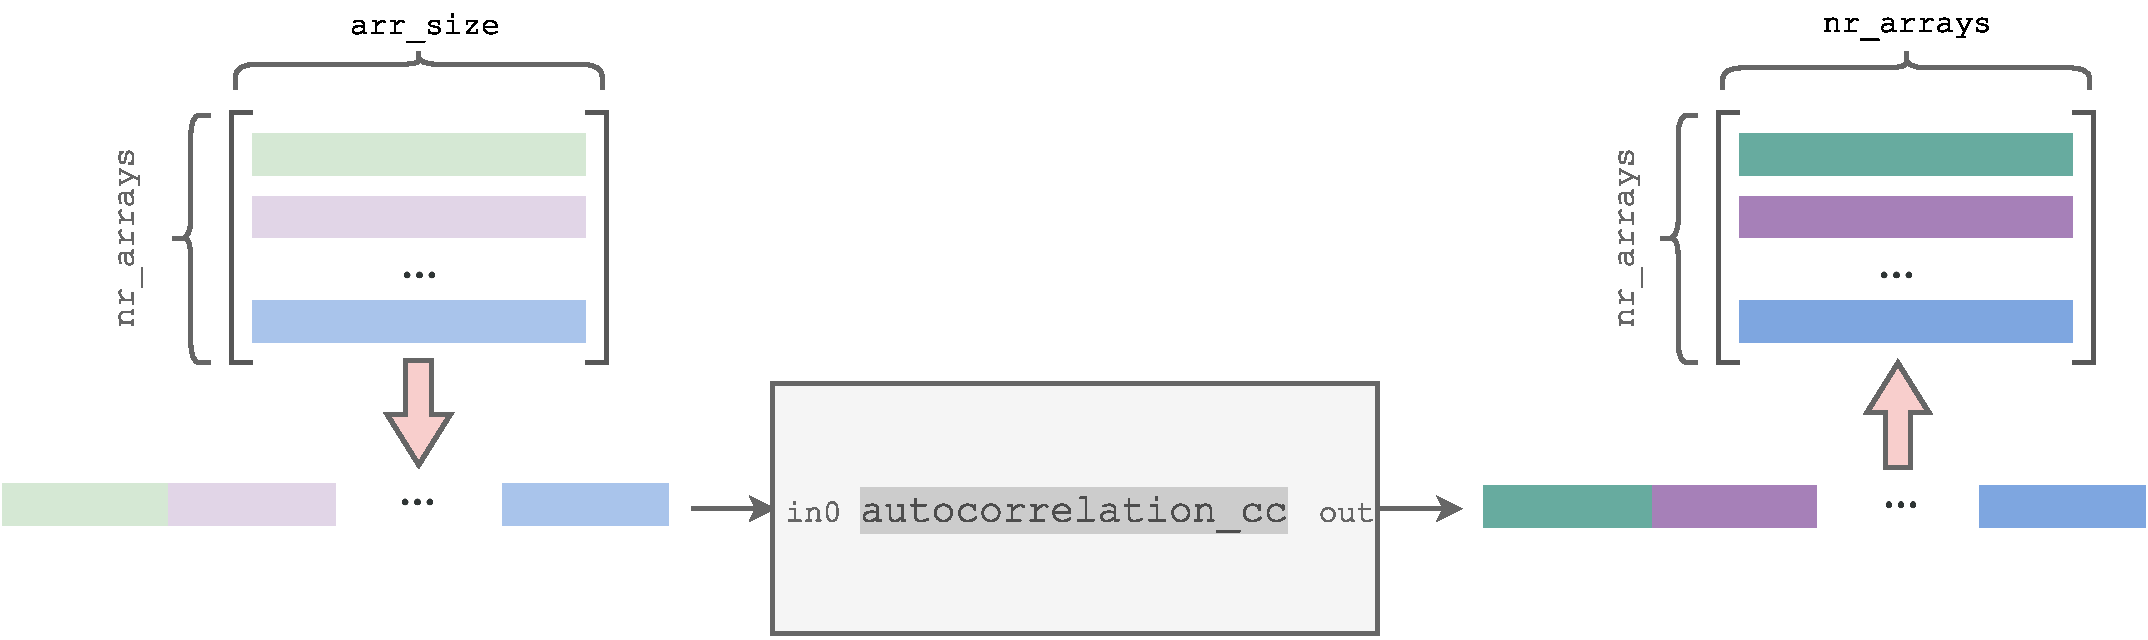
\includegraphics[width=1\textwidth]{src/img/autocorrelation-block}
    \caption{Structura intrărilor si ieșirilor blocului GNU Radio care
    realizează autocorelația}
    \label{fig:autocorrelation-block}
\end{figure}

În programul principal, putem să citim un număr de reducții necesar formării
unui element de ieșire și să procesăm acest element de ieșire în timpul în
care se calculează următorul, efectuând, în acest mod, o ușoară paralelizare. \\

Acest bloc nu este atât de sensibil la erorile de precizie, atingând cu el
același nivel de acuratețe a estimării unghiului de incidență ca și în cazul
implementării originale.
